\documentclass{mathnote_cmyk}
\usepackage{mathnote_cmyk}

% 製本用：表紙の裏・裏表紙の裏は完全な白紙にする
\MathNoteVersoLabelfalse
% 製本用：総ページ数（表紙・裏表紙を含む）．4 の倍数にしておく
\newcommand{\BookTotalPages}{36}

\begin{document}

% タイトルページの呼び出し
\tituloum
  {Analysis}
  {Namachan}
  {Mathematics Notes}
  {An introduction to limits, differentiation, and integration}
  {\today}

%\include{Preambulo/Capa}

\cleardoublepage
\pagenumbering{arabic}
\pagecolor{white}

% 目次
\localtableofcontents

\phantomsection
\part{数}

\begin{abstract}
この章では，解析学の議論の土台となる「数」に関する用語や概念を整理する．まず高校までに学んだ数の体系を振り返り，自然数から複素数へと数を拡張してきた動機を確認する．次に，実数の順序構造に注目し，最大元・最小元，上界・下界といった概念を定義する．そのうえで，最大元・最小元の一般化として上限・下限を導入し，その判定条件をいくつかの形で与える．これらの概念は，\partref{実数の連続性}で「実数の連続性」を述べるための言葉として不可欠なものである．
\end{abstract}

\phantomsection
\section{実数}

\phantomsection
\subsection{数の種類}

解析学を学ぶにあたって，大学の講義ではまず「数列の極限」を定義し直すことから始めることが多い．
大学で学ぶ「実数列の収束」の定義（\partref{極限}）は，次のようなものである：
\begin{quotation}
  実数列$(a_n)_{n \in \mathbb{N}}$が$a \in \mathbb{R}$に収束するとは，次が成り立つことである：

  任意の$\varepsilon > 0$に対して，ある$n_0 \in \mathbb{N}$が存在し，すべての$n \in \mathbb{N}$に対して$n \geqq n_0$ならば
  \[
    \abs{a_n - a} < \varepsilon
  \]
  が成り立つ．
\end{quotation}
この定義は，いわゆる\emph{$\varepsilon$--$N$論法}とよばれるものであり，高校で学んだ「数列がある値に限りなく近づく」という直感的な説明を厳密に表現したものである．
この定義を正確に理解するためにも，まずは「数」についていくつかの用語を定義することから始めよう．

まず，高校で学んできた「数」を振り返ってみよう．

\begin{reviewbox}[数の集合]
  \small
  \begin{tabular}{@{}p{14\zw}@{\hspace{1.5\zw}}l@{}}
    自然数（natural numbers）&
    $\mathbb{N} = \{1,2,3,\ldots\}$\footnotemark\\[0.35\baselineskip]

    整数（integers）&
    $\mathbb{Z} = \{\ldots,-2,-1,0,1,2,\ldots\}$\\[0.35\baselineskip]

    有理数（rational numbers）&
    $\mathbb{Q} = \left\{ \frac{a}{b} \relmiddle| a \in \mathbb{Z},\ b \in \mathbb{N} \right\}$\\[0.35\baselineskip]

    実数（real numbers）&
    $\mathbb{R}$\\[0.35\baselineskip]

    複素数（complex numbers）&
    $\mathbb{C} = \{ a + bi \mid a,b \in \mathbb{R} \}$
  \end{tabular}
  \footnotetext{自然数に$0$を含める流儀もあるが，本書では自然数に$0$を含めないものとする．}
\end{reviewbox}

高校まではあまりなかった視点かもしれないが，ここで少し考察に付き合ってほしい．
$m,n \in \mathbb{N}$とすると，$m+n \in \mathbb{N}$かつ$mn \in \mathbb{N}$である．
大学で学ぶ言葉を使うと，このことを「$\mathbb{N}$は加法と乗法に関して\emph{閉じている}」という\footnote{一般に，ある集合の元どうしで演算を行った結果がつねにその集合の元になるとき，その集合はその演算に関して閉じているという．}．
しかし，$n-m$や$n \div m$は$\mathbb{N}$に属さない場合がある（たとえば$2-3$や$2 \div 3$）．

そこで，自然数を拡張して整数を，さらに有理数を導入したのであった．
実際，任意の$a,b \in \mathbb{Q}$に対して
\[
  a + b \in \mathbb{Q},\quad a - b \in \mathbb{Q},\quad ab \in \mathbb{Q},\quad a \div b \in \mathbb{Q}~(b \ne 0)
\]
が成り立つ．このように，有理数は加法・減法・乗法・除法に関して閉じている．

しかし，$\mathbb{Q}$に属さない数もある．たとえば$\sqrt{2}$は有理数ではない．さらに，数列
\[
  a_n = \left( 1+\frac{1}{n} \right)^n
\]
を考えると，各$n \in \mathbb{N}$について$a_n \in \mathbb{Q}$であるにもかかわらず，
\[
  \lim_{n \to \infty} \left(1+\frac{1}{n}\right)^n = e \in \mathbb{R} \setminus \mathbb{Q}
\]
となり，極限として無理数が現れる．つまり，有理数列の極限が無理数になる場合もあるのである．

このような事情をふまえ，実数全体の集合$\mathbb{R}$については，空でない部分集合$A \subset \mathbb{R}$が上に有界ならば$A$の上限$\sup A$が$\mathbb{R}$に存在することを，\emph{実数の連続性の公理}として認めることにする\footnote{同様に，空でない部分集合$A \subset \mathbb{R}$が下に有界ならば，$A$の下限$\inf A$も$\mathbb{R}$に存在する．上限・下限は本章で定義し，この公理は\partref{実数の連続性}で改めて述べる．}．

さらに，$i^2 = -1$を満たす数$i$を導入して，複素数全体の集合$\mathbb{C}$を構成する．
このようにして，自然数$\mathbb{N}$，整数$\mathbb{Z}$，有理数$\mathbb{Q}$，実数$\mathbb{R}$，複素数$\mathbb{C}$という数の体系が構築される．

これらをふまえて「数」に関する議論を厳密に進めていきたいが，そのためにはいくつかの用語を定義する必要がある．
そこでまずは「慣れ親しんだ集合」として，$\mathbb{R}$の部分集合$A$を中心に議論を進めていこう．

\phantomsection
\subsection{実数の順序構造}

\begin{prop}{実数の稠密性}{real_dense}
  任意の$a,b \in \mathbb{R}$に対して，$a < b$ならば
  \[
    a < c < b
  \]
  を満たす$c \in \mathbb{R}$が存在する．
\end{prop}

\begin{tleftbar}
  \begin{proof}
    $c = (a+b)/2$とおけば，これは$a < c < b$を満たす．これが証明すべきことであった．
  \end{proof}
\end{tleftbar}

\prref{real_dense}の証明では，やや天下り的に「$c = (a+b)/2$とおけばよい」と書いた．
理由をいっさい述べることなくこのような数をとったが，このように$c$を選ぶと都合がよいことは，数直線上で$a$と$b$のちょうど真ん中にある数を選んでいると考えれば自然に理解できる．

もちろん，$c$の選び方はひと通りではない．
たとえば$0 < a < b$のときは，$a$と$b$の対数平均
\[
  c = \frac{b-a}{\log b - \log a}
\]
をとっても，$a < c < b$が成り立つ．
また，証明において重要なのは，条件を満たす$c$が少なくとも$1$つ存在することを示すことであり，その$c$をどのように発見したかまで説明する必要はない．

\begin{prop}{任意の正数より小さい非負実数}{nonnegative_less_than_all_positive}
  $a \geqq 0$とする．
  任意の$\varepsilon > 0$に対して$a < \varepsilon$が成り立つならば，$a = 0$である．
\end{prop}

\begin{tleftbar}
  \begin{proof}
    背理法で示す．$a \ne 0$と仮定する．
    $a \geqq 0$であるから，このとき$a > 0$である．

    \prref{real_dense}より，$0 < \varepsilon < a$を満たす$\varepsilon \in \mathbb{R}$が存在する．
    とくに$\varepsilon > 0$であるから，仮定より$a < \varepsilon$でなければならない．
    これは$\varepsilon < a$に矛盾する．

    したがって，$a = 0$である．これが証明すべきことであった．
  \end{proof}
\end{tleftbar}

\begin{remark}[「任意の$\varepsilon>0$」の読み方]
  「任意の$\varepsilon > 0$に対して$a < \varepsilon$が成り立つ」とは，ある特定の$\varepsilon$に対してのみ成り立つという意味ではなく，どれほど小さい正数$\varepsilon$をとっても$a < \varepsilon$が成り立つという意味である．
  たとえば，$a = 1$として$\varepsilon = 2$をとれば確かに$a < \varepsilon$となるが，これは仮定を満たすことを意味しない．実際，$\varepsilon = 1/2$とすれば$a < \varepsilon$は成り立たない．
  このように，$a > 0$である限り，$a$より小さい正数$\varepsilon$をとれば必ず仮定に反する．
\end{remark}

ここまでは，実数どうしの大小関係について考えてきた．
次に，ある集合の中で「最も大きい元」や「最も小さい元」を考える．
このような元を，それぞれ最大元・最小元という．

\begin{definition}{最大元・最小元}{最大元・最小元}
  $A \subset \mathbb{R}$とする．

  $m \in \mathbb{R}$が
  \[
    \begin{cases}
      \textup{(1)}\ m \in A,\\
      \textup{(2)}\ \lall{x \in A} \lst x \leqq m
    \end{cases}
  \]
  を満たすとき，$m$を$A$の\emph{最大元}\index{さいだいげん@最大元}といい，
  \[
    m = \max A
  \]
  とかく．

  また，$m \in \mathbb{R}$が
  \[
    \begin{cases}
      \textup{(1)}\ m \in A,\\
      \textup{(2)}\ \lall{x \in A} \lst m \leqq x
    \end{cases}
  \]
  を満たすとき，$m$を$A$の\emph{最小元}\index{さいしょうげん@最小元}といい，
  \[
    m = \min A
  \]
  とかく．
\end{definition}

\begin{remark}[最大元と最大値]
  「最大元」と似た言葉に「最大値」がある．
  これらは密接に関係しているが，何について述べているかが異なる．
  最大元は，集合そのものに対して定めた言葉である．
  一方，関数$f \colon D \to \mathbb{R}$について「$f$の最大値」というときは，$f$の値全体の集合
  \[
    f(D) = \{f(x) \mid x \in D\}
  \]
  の最大元のことをいう．
  すなわち
  \[
    \max_{x \in D} f(x) \coloneqq \max f(D)
  \]
  であり，関数の最大値は，その値全体の集合の最大元として捉えることができる．
  この意味で，本書では，関数については最大値，集合については最大元という語を用いる\footnote{%
    ただし，$\max A,\min A$を「$A$の最大値」「$A$の最小値」とよぶことも広く行われており，これらが誤りというわけではない．%
  }．
  最小値と最小元についても同様である．

  なお，$\max_{x \in D} f(x)$は最大値であって，$D$の元ではない．
  これに対し，$f(a) = \max f(D)$を満たす$a \in D$を，$f$が最大値をとる点という．
  最大値は存在すればただひとつに定まるのに対し，最大値をとる点は複数存在しうる．
  たとえば$f(x) = x^{2}$，$D = [-1,1]$のとき，最大値は$1$であるが，これをとる点は$x = 1$と$x = -1$の$2$つである．
\end{remark}

\begin{figure}[htbp]
  \centering
  \begin{tikzpicture}[scale=1.0, >=stealth]

    % ==================================================
    % A = (0,1]
    % ==================================================

    % 数直線
    \draw[->, thick, black] (-0.5,1.3) -- (5.2,1.3);

    % 集合 A
    \draw[line width=2pt, figaccent] (1,1.3) -- (4,1.3);

    % 端点
    % 0: A に含まれない
    \draw[thick, figaccent, fill=white] (1,1.3) circle (2.5pt);
    % 1: A に含まれる
    \filldraw[figaccent] (4,1.3) circle (2.5pt);

    % 目盛り
    \node[below] at (1,1.15) {$0$};
    \node[below] at (4,1.15) {$1$};

    % 集合名（線と重ならないように左上へ）
    \node[above left] at (-0.25,1.3) {$A$};

    % 最大元
    \node[above, figaccent] at (4,1.45) {最大元};

    % 補足
    \node[right, align=left] at (5.4,1.3)
      {$A=(0,1]$\\最小元は存在しない};

    % ==================================================
    % B = [0,1)
    % ==================================================

    % 数直線
    \draw[->, thick, black] (-0.5,-0.2) -- (5.2,-0.2);

    % 集合 B
    \draw[line width=2pt, figaccent] (1,-0.2) -- (4,-0.2);

    % 端点
    % 0: B に含まれる
    \filldraw[figaccent] (1,-0.2) circle (2.5pt);
    % 1: B に含まれない
    \draw[thick, figaccent, fill=white] (4,-0.2) circle (2.5pt);

    % 目盛り
    \node[below] at (1,-0.35) {$0$};
    \node[below] at (4,-0.35) {$1$};

    % 集合名（線と重ならないように左上へ）
    \node[above left] at (-0.25,-0.2) {$B$};

    % 最小元
    \node[above, figaccent] at (1,-0.05) {最小元};

    % 補足
    \node[right, align=left] at (5.4,-0.2)
      {$B=[0,1)$\\最大元は存在しない};

  \end{tikzpicture}
  \caption{最大元・最小元のイメージ}
\end{figure}

最大元・最小元は，単に集合の「端」にある数ではなく，その集合自身に属していなければならない．
したがって，集合に上端や下端が見えていても，その点が集合に含まれていなければ最大元・最小元は存在しない．

\begin{example}{最大元・最小元の例}{最大元・最小元の例}
  集合$A = \{x \in \mathbb{R} \mid 0 < x \leqq 1\}$に対して，$\max A = 1$であり，$\min A$は存在しない．
  また，集合$B = \{x \in \mathbb{R} \mid 0 \leqq x < 1\}$に対して，$\min B = 0$であり，$\max B$は存在しない．
\end{example}

\begin{prop}{最大元・最小元の一意性}{max_min_uniqueness}
  $A \subset \mathbb{R}$とする．$A$の最大元・最小元は，存在すればただひとつである．
\end{prop}

\begin{tleftbar}
  \begin{proof}
    $m,m'$がともに$A$の最大元であると仮定する．
    最大元の定義より，
    \[
      m = \max A
      \quad\lequiv\quad
      \begin{cases}
        \textup{(1)}\ m \in A,\\
        \textup{(2)}\ \lall{x \in A} \lst x \leqq m
      \end{cases}
    \]
    であり，同様に
    \[
      m' = \max A
      \quad\lequiv\quad
      \begin{cases}
        \textup{(1)}\ m' \in A,\\
        \textup{(2)}\ \lall{x \in A} \lst x \leqq m'
      \end{cases}
    \]
    である．

    $m$は$A$の最大元であり，$m' \in A$であるから，
    \[
      m' \leqq m
    \]
    が成り立つ．また，$m'$は$A$の最大元であり，$m \in A$であるから，
    \[
      m \leqq m'
    \]
    が成り立つ．したがって，$m = m'$である．

    最小元についても同様にして一意性が示される．これが証明すべきことであった．
  \end{proof}
\end{tleftbar}

\begin{remark}[一意性と記号の正当化]
  ところで，なぜわざわざ一意性を確認しなければならないのだろうか．
  それは，\deref{最大元・最小元}において$m = \max A$という「記号」を導入したからである．

  一般に，数学において記号を定めるときは，その記号が指し示す対象がただひとつに定まっていなければならない．
  たとえば，空集合を表す記号$\varnothing$は，「元をもたない集合はただひとつしかない」という事実に支えられて初めて意味をもつ．
  また，正則行列$A$の逆行列を$A^{-1}$とかくのも，「$AB = BA = E$を満たす行列$B$は存在すればただひとつである」ことが証明されているからこそ許される記法である．
  もし条件を満たす対象が複数ありうるならば，記号がそのうちのどれを指しているのかが定まらず，たとえば$\max A = 1$のような等式は意味をなさなくなってしまう．
  \prref{max_min_uniqueness}は，記号$\max A,\min A$の使用を正当化するための命題なのである．

  別の見方をすれば，$\max$は「集合$A$を入力すると実数$\max A$を返す対応」，すなわち一種の写像とみなすこともできる%
  \footnote{ただし，最大元が存在しない集合には値を定めないので，正確には「最大元をもつ集合全体」を定義域とする写像である．}．
  写像とは，入力ひとつに対して出力を\textbf{ただひとつ}定める対応のことであった．
  したがって，$\max$をこのような写像として扱うためにも，最大元の一意性が保証されていなければならない．
  最小元$\min$についても同様である．
\end{remark}

ただし，最大元や最小元は，$\mathbb{R}$の部分集合に対してつねに存在するとは限らない．
そこで，$[0,1)$や$(0,1]$のような最大元（最小元）をもたない集合に対しても，似た概念を与えたい．
「最大元」と「最小元」に似た概念として，「上限」と「下限」を定義しよう．
そのために，まず上界・下界を定義する．

\begin{definition}{上界・下界・有界}{上界・下界・有界}
  $A \subset \mathbb{R}$とする．

  $a \in \mathbb{R}$が
  \[
    \lall{x \in A} \lst x \leqq a
  \]
  を満たすとき，$a$を$A$の\emph{上界}\index{じょうかい@上界}という．
  $A$の上界が存在するとき，$A$は\emph{上に有界}であるという．
  また，$A$の上界全体の集合を$U(A)$とかく．すなわち，
  \[
    U(A) = \{ a \in \mathbb{R} \mid \lall{x \in A} \lst x \leqq a \}
  \]
  である．

  同様に，$a \in \mathbb{R}$が
  \[
    \lall{x \in A} \lst a \leqq x
  \]
  を満たすとき，$a$を$A$の\emph{下界}\index{かかい@下界}という．
  $A$の下界が存在するとき，$A$は\emph{下に有界}であるという．
  また，$A$の下界全体の集合を$L(A)$とかく．すなわち，
  \[
    L(A) = \{ a \in \mathbb{R} \mid \lall{x \in A} \lst a \leqq x \}
  \]
  である．

  そして，$A$が上にも下にも有界であるとき，$A$は\emph{有界}\index{ゆうかい@有界}であるという．
\end{definition}

\deref{上界・下界・有界}は難解に思えるかもしれない．
いわんとしていることは，「$U(A)$は，$A$のどの元よりも大きいかまたは等しい数全体の集合」ということである．
具体例で説明しよう．

\begin{example}{上界・下界の例}{上界・下界の例}
  集合
  \[
    A = \{ x \in \mathbb{R} \mid 0 < x < 1 \}
  \]
  について，
  \[
    U(A) = [1,\infty),
    \quad
    L(A) = (-\infty,0]
  \]
  である．
  とくに，集合$A$は有界である．
\end{example}

\begin{prop}{有界であるための必要十分条件}{boundedness_characterization}
  $A \subset \mathbb{R}$とする．
  $A$が上に有界であるための必要十分条件は，$U(A) \ne \varnothing$である．
  また，$A$が下に有界であるための必要十分条件は，$L(A) \ne \varnothing$である．
\end{prop}

\begin{tleftbar}
  \begin{proof}
    まず，上に有界であることについて示す．

    $A$が上に有界であるとする．
    このとき，$A$の上界が存在するので，$U(A) \ne \varnothing$である．

    逆に，$U(A) \ne \varnothing$であるとする．
    このとき，ある$a \in U(A)$が存在する．
    $U(A)$の定義より，すべての$x \in A$に対して$x \leqq a$である．
    したがって，$a$は$A$の上界であるから，$A$は上に有界である．

    下に有界であることについても同様に議論すると，$A$が下に有界であるための必要十分条件が$L(A) \ne \varnothing$であることがわかる．これが証明すべきことであった．
  \end{proof}
\end{tleftbar}

\begin{prop}{有界であるための必要十分条件（上下）}{boundedness_characterization_both}
  $A \subset \mathbb{R}$とする．
  $A$が有界であるための必要十分条件は，$U(A) \ne \varnothing$かつ$L(A) \ne \varnothing$である．
\end{prop}

\begin{tleftbar}
  \begin{proof}
    $A$が有界であるとする．
    このとき，\deref{上界・下界・有界}により$A$は上に有界であるから，\prref{boundedness_characterization}により$U(A) \ne \varnothing$である．
    同様に，$A$は下に有界であるから，\prref{boundedness_characterization}により$L(A) \ne \varnothing$である．

    逆に，$U(A) \ne \varnothing$かつ$L(A) \ne \varnothing$であるとする．
    このとき，\prref{boundedness_characterization}により$A$は上にも下にも有界である．
    したがって，$A$は有界である．これが証明すべきことであった．
  \end{proof}
\end{tleftbar}

\begin{example}{有界な集合}{有界な集合}
  集合
  \[
    A = \{ x \in \mathbb{R} \mid x > 1 \}
  \]
  は下に有界であるが，上に有界ではない．

  一方，集合
  \[
    B = \{ x \in \mathbb{R} \mid 1 < x < 4 \}
  \]
  は上にも下にも有界である．したがって，$B$は有界である．
\end{example}

\begin{definition}{上限と下限}{sup_inf}
  $A$を$\mathbb{R}$の空でない部分集合とする．

  $A$が上に有界であるとき，
  \[
    \sup A = \min U(A)
  \]
  と定める．このとき，$\sup A$を$A$の\emph{最小上界}または\emph{上限}\index{じょうげん@上限}という．

  また，$A$が下に有界であるとき，
  \[
    \inf A = \max L(A)
  \]
  と定める．このとき，$\inf A$を$A$の\emph{最大下界}または\emph{下限}\index{かげん@下限}という．
\end{definition}

% --- TikZ による図解 ---
\begin{figure}[htbp]
  \centering
  \begin{tikzpicture}[scale=0.8, >=stealth]
    % ==================================================
    % 領域
    % ==================================================
    % 下界・上界の領域を薄いアクセント色で表示
    \fill[figaccent!8] (-7,0) rectangle (-2,1);
    \fill[figaccent!8] (2,0) rectangle (7,1);
    % 集合 A の領域
    \fill[black!7] (-2,0) rectangle (2,1);
    % ==================================================
    % 数直線
    % ==================================================
    \draw[->, thick, black]
      (-7.5,0) -- (7.5,0)
      node[right] {$\mathbb{R}$};
    % ==================================================
    % inf A, sup A
    % ==================================================
    % 下限
    \draw[figaccent, thick]
      (-2,0) -- (-2,1.2)
      node[above] {$\inf A$};
    % 上限
    \draw[figaccent, thick]
      (2,0) -- (2,1.2)
      node[above] {$\sup A$};
    % 境界点
    \filldraw[figaccent] (-2,0) circle (2pt);
    \filldraw[figaccent] ( 2,0) circle (2pt);
    % ==================================================
    % 上界・下界を表す上辺
    % ==================================================
    \draw[thick, black]
      (-7,1) -- (-2,1);
    \draw[thick, black]
      (2,1) -- (7,1);
    % ==================================================
    % ラベル
    % ==================================================
    % 集合 A
    \node at (0,0.5) {$A$};
    % 下界全体
    \node[figaccent] at (-4.5,0.5)
      {$L(A)$（下界）};
    % 上界全体
    \node[figaccent] at (4.5,0.5)
      {$U(A)$（上界）};
  \end{tikzpicture}
  \caption{上限・下限と上界・下界のイメージ}
\end{figure}

\begin{remark}[上限・下限の一意性]
  ここで，上限・下限の一意性について確認しておこう．
  \deref{sup_inf}によれば，$\sup A$は上界全体の集合$U(A)$の最小元として，$\inf A$は下界全体の集合$L(A)$の最大元として定義されている．
  そして，\prref{max_min_uniqueness}により，最大元・最小元は存在すればただひとつであった．
  したがって，$\sup A$および$\inf A$も存在すればただひとつである（上限・下限の一意性）．
  すなわち，上限・下限の一意性は，新たに証明し直すまでもなく，最大元・最小元の一意性から直ちに従う．
  これにより，記号$\sup A,\inf A$の使用もまた正当化されるのである．
\end{remark}

\begin{theorem}{上限・下限の判定条件}{characterization}
  $A$を$\mathbb{R}$の空でない部分集合とする．

  $A$が上に有界であるとき，$m \in \mathbb{R}$について
  \[
    m = \sup A
    \quad\lequiv\quad
    \begin{cases}
      \textup{(1)}\ \lall{x \in A} \lst x \leqq m,\\
      \textup{(2)}\ \lall{a < m} \lsep \lex{x \in A} \lst a < x
    \end{cases}
  \]
  が成り立つ．

  また，$A$が下に有界であるとき，$m \in \mathbb{R}$について
  \[
    m = \inf A
    \quad\lequiv\quad
    \begin{cases}
      \textup{(1)}\ \lall{x \in A} \lst m \leqq x,\\
      \textup{(2)}\ \lall{a > m} \lsep \lex{x \in A} \lst x < a
    \end{cases}
  \]
  が成り立つ．
\end{theorem}

\begin{tleftbar}
  \begin{proof}
    まず，上限の場合を示す．$A$の上界全体の集合を$U(A)$とする．
    上限の定義より，
    \[
      m = \sup A
      \quad\lequiv\quad
      m = \min U(A)
    \]
    である．

    さらに，最小元の定義より，
    \[
      m = \min U(A)
      \quad\lequiv\quad
      \begin{cases}
        \textup{(1)}\ m \in U(A),\\
        \textup{(2)}\ \lall{a \in U(A)} \lst m \leqq a
      \end{cases}
    \]
    である．ここで，(2)の対偶をとると，
    \[
      \lall{a \in U(A)} \lst m \leqq a
      \quad\lequiv\quad
      \lall{a \in \mathbb{R}} \lst (a < m \limp a \notin U(A))
    \]
    である．したがって，
    \[
      m = \sup A
      \quad\lequiv\quad
      \begin{cases}
        \textup{(1)}\ m \in U(A),\\
        \textup{(2)}\ \lall{a < m} \lst a \notin U(A)
      \end{cases}
    \]
    となる．

    最後に，上界の定義より，
    \[
      m \in U(A)
      \quad\lequiv\quad
      \lall{x \in A} \lst x \leqq m
    \]
    であり，また
    \[
      a \notin U(A)
      \quad\lequiv\quad
      \lex{x \in A} \lst a < x
    \]
    である．ゆえに，
    \[
      m = \sup A
      \quad\lequiv\quad
      \begin{cases}
        \textup{(1)}\ \lall{x \in A} \lst x \leqq m,\\
        \textup{(2)}\ \lall{a < m} \lsep \lex{x \in A} \lst a < x
      \end{cases}
    \]
    が成り立つ．

    下限の場合も同様である．$A$の下界全体の集合を$L(A)$とすると，
    \[
      m = \inf A
      \quad\lequiv\quad
      m = \max L(A)
    \]
    である．最大元の定義より，
    \[
      m = \max L(A)
      \quad\lequiv\quad
      \begin{cases}
        \textup{(1)}\ m \in L(A),\\
        \textup{(2)}\ \lall{a \in L(A)} \lst a \leqq m
      \end{cases}
    \]
    である．(2)の対偶をとると，
    \[
      \lall{a \in L(A)} \lst a \leqq m
      \quad\lequiv\quad
      \lall{a \in \mathbb{R}} \lst (m < a \limp a \notin L(A))
    \]
    である．

    ここで，下界の定義より，
    \[
      m \in L(A)
      \quad\lequiv\quad
      \lall{x \in A} \lst m \leqq x
    \]
    であり，また
    \[
      a \notin L(A)
      \quad\lequiv\quad
      \lex{x \in A} \lst x < a
    \]
    である．したがって，
    \[
      m = \inf A
      \quad\lequiv\quad
      \begin{cases}
        \textup{(1)}\ \lall{x \in A} \lst m \leqq x,\\
        \textup{(2)}\ \lall{a > m} \lsep \lex{x \in A} \lst x < a
      \end{cases}
    \]
    が成り立つ．これが証明すべきことであった．
  \end{proof}
\end{tleftbar}

\begin{theorem}{$\varepsilon$を用いた特徴づけ}{epsilon_delta}
  $A$を$\mathbb{R}$の空でない部分集合とする．

  $A$が上に有界であるとき，$m \in \mathbb{R}$について
  \[
    m = \sup A
    \quad\lequiv\quad
    \begin{cases}
      \textup{(1)}\ \lall{x \in A} \lst x \leqq m,\\
      \textup{(2)}\ \lall{\varepsilon > 0} \lsep \lex{a \in A} \lst m - \varepsilon < a
    \end{cases}
  \]
  が成り立つ．

  また，$A$が下に有界であるとき，$m \in \mathbb{R}$について
  \[
    m = \inf A
    \quad\lequiv\quad
    \begin{cases}
      \textup{(1)}\ \lall{x \in A} \lst m \leqq x,\\
      \textup{(2)}\ \lall{\varepsilon > 0} \lsep \lex{a \in A} \lst a < m + \varepsilon
    \end{cases}
  \]
  が成り立つ．
\end{theorem}

\begin{example}{集合$A=[0,1)$の上限・下限}{sup_inf_ex}
  集合$A \coloneqq [0,1)$の上限$\sup A$と下限$\inf A$を，本節で導入した$3$通りの視点から求めよう．

  \begin{description}
    \item[(1) 上界・下界全体の集合による定義（\deref{上界・下界・有界}，\deref{sup_inf}）]\mbox{}\\
      まず，上界全体の集合$U(A)$を求める．任意の$a \in A$に対して$a < 1$であるから，$1$は$A$の上界である．よって$1 \in U(A)$となる．
      次に$x < 1$とし，$a \coloneqq \max\{0,(x+1)/2\}$とおく．このとき$a \in A$かつ$x < a$であるから，$x$は$A$の上界ではない．
      これより$U(A) = [1, \infty)$であり，その最小元が上限であるから，$\sup A = \min U(A) = 1$を得る．

      同様に，下界全体の集合$L(A)$を求める．任意の$a \in A$に対して$a \geqq 0$であるから，$0$は$A$の下界である．よって$0 \in L(A)$となる．
      次に$y > 0$とし，$a \coloneqq \min\{y/2,1/2\}$とおく．このとき$a \in A$かつ$a < y$であるから，$y$は$A$の下界ではない．
      これより$L(A) = (-\infty, 0]$であり，その最大元が下限であるから，$\inf A = \max L(A) = 0$を得る．

    \item[(2) 上限・下限の判定条件（\thref{characterization}）]\mbox{}\\
      $m = 1$とおく．任意の$a \in A$に対して$a < 1$であるから，\thref{characterization}の(1)が成り立つ．
      また，$x < 1$とすると，$a \coloneqq \max\{0,(x+1)/2\}$は$a \in A$かつ$x < a$を満たすから，(2)も成り立つ．
      よって，\thref{characterization}より$\sup A = 1$である．

      $m = 0$とおく．任意の$a \in A$に対して$a \geqq 0$であるから，(1)が成り立つ．
      また，$x > 0$とすると，$a \coloneqq \min\{x/2,1/2\}$は$a \in A$かつ$a < x$を満たすから，(2)も成り立つ．
      よって，\thref{characterization}より$\inf A = 0$である．

    \item[(3) $\varepsilon$を用いた特徴づけ（\thref{epsilon_delta}）]\mbox{}\\
      $m = 1$とおく．任意の$a \in A$に対して$a \leqq 1$であるから，\thref{epsilon_delta}の(1)が成り立つ．
      また，任意の$\varepsilon > 0$に対して，$a \in A$を
      \[
        a \coloneqq
        \begin{cases}
          1 - \dfrac{\varepsilon}{2} & (0 < \varepsilon \leqq 1), \\[6pt]
          0 & (\varepsilon > 1)
        \end{cases}
      \]
      と定めれば，いずれの場合も$1 - \varepsilon < a$が成り立つから，(2)も成り立つ．
      よって，\thref{epsilon_delta}より$\sup A = 1$である．

      $m = 0$とおく．任意の$a \in A$に対して$a \geqq 0$であるから，(1)が成り立つ．
      また，任意の$\varepsilon > 0$に対して$a \coloneqq \min\{\varepsilon/2,1/2\}$とおけば，$a \in A$かつ$a < 0 + \varepsilon$が成り立つから，(2)も成り立つ．
      よって，\thref{epsilon_delta}より$\inf A = 0$である．
  \end{description}

  以上より，
  \[
    \sup A = 1, \quad \inf A = 0
  \]
  を得る．どの視点から求めても同じ結論に到達することを確認してほしい．
\end{example}

\phantomsection
\part{極限}

\begin{abstract}
この章では，実数列の極限を厳密に定義し，その基本性質を確認する．高校で数列の極限を定義する際に用いた「限りなく近づく」という表現は，厳密な議論を行ううえでは曖昧さを残すものである．そこでまず，この表現を論理的に厳密な形に定義し直した$\varepsilon$--$N$論法を導入し，実数列の収束と発散を定義する．次に，数列を自然数全体から実数全体への写像として捉え直し，極限の一意性を証明する．そのうえで，極限の四則演算や，極限操作が順序関係を保存することを示し，数列の収束を判定する強力な手法である「はさみうちの原理」を具体例とともに確認しよう．ここで扱う議論は，\partref{実数の連続性}で「実数の連続性」を数学的に記述するための準備にもなる．
\end{abstract}

\phantomsection
\section{実数列の極限}\label{sec:実数列の極限}

\phantomsection
\subsection{実数列の性質}

高校数学において，数列の極限は次のように定義されていた．

\begin{quotation}
  数列$(a_n)_{n \in \mathbb{N}}$\footnote{高校数学では数列を$\{a_n\}$と表記することが多いが，本書では$n$が自然数を動くことを明示するために$(a_n)_{n \in \mathbb{N}}$とかく．
  また，$\{a_n\}$という記法は集合$\{ a_n \mid n \in \mathbb{N} \}$と混同しやすい．たとえば$a_n \coloneqq (-1)^n$のとき，数列としては各項が振動するが，集合としては$\{ -1, 1 \}$という$2$つの元からなる集合を指すことになる．}において，番号$n$を限りなく大きくするとき，$a_n$の値がある一定の値$a$に限りなく近づくならば，この数列は$a$に収束するといい，
  \[
    \lim_{n \to \infty} a_n = a
  \]
  とかく．
\end{quotation}

しかし，この「限りなく大きくする」「限りなく近づく」といった表現は，直感的ではあるものの，数学的に厳密な定義とはいいがたい．何をもって「限りなく」とするのか，その基準が曖昧だからである．
こうした直感的な表現を排し，論理的に厳密な形で実数列\footnote{各項が実数である数列のこと．}の収束を定義し直したものが，次の$\varepsilon$--$N$論法である．

\begin{definition}{実数列の収束}{実数列の収束}
  実数列$(a_n)_{n \in \mathbb{N}}$が$a \in \mathbb{R}$に\emph{収束する}\index{じっすうれつのしゅうそく@実数列の収束}とは，次が成り立つことである：

  任意の$\varepsilon > 0$に対して，ある$n_0 \in \mathbb{N}$が存在し，すべての$n \in \mathbb{N}$に対して$n \geqq n_0$ならば
  \[
    \abs*{a_n - a} < \varepsilon
  \]
  が成り立つ．
  このとき，$a$を$(a_n)_{n \in \mathbb{N}}$の\emph{極限}\index{きょくげん@極限}といい，
  \[
    \lim_{n \to \infty} a_n = a
    \quad\text{または}\quad
    a_n \to a~(n \to \infty)
  \]
  とかく．

  これを論理記号でかけば，次のようになる：
  \[
    \lall{\varepsilon > 0} \lsep \lex{n_0 \in \mathbb{N}} \lsep \lall{n \in \mathbb{N}} \lst
    \bigl( n \geqq n_0 \limp \abs*{a_n - a} < \varepsilon \bigr)
  \]
\end{definition}

\begin{remark}[日本語の言い回しと論理式の対応]
  \deref{実数列の収束}の$2$つの表現は，次のように$1$対$1$に対応している．
  \begin{center}
    \begin{tabular}{l|l}
      \hline
      日本語による表現                                  & 論理記号による表現                              \\
      \hline
      任意の$\varepsilon > 0$に対して                   & $\lall{\varepsilon > 0}$                        \\
      ある$n_0 \in \mathbb{N}$が存在し                  & $\lex{n_0 \in \mathbb{N}}$                      \\
      すべての$n \in \mathbb{N}$に対して                & $\lall{n \in \mathbb{N}}$                       \\
      $n \geqq n_0$ならば$\abs{a_n - a} < \varepsilon$  & $n \geqq n_0 \limp \abs{a_n - a} < \varepsilon$ \\
      \hline
    \end{tabular}
  \end{center}

  とくに本質的なのは，$\lall{\varepsilon > 0}$が$\lex{n_0 \in \mathbb{N}}$より\textbf{前}にあることである．
  この順序は「どんなに小さな$\varepsilon$を指定されても，それに応じて$n_0$を選び直してよい」ことを表しており，$n_0$は$\varepsilon$に依存してよい．
  順序を入れ替えて$\lex{n_0 \in \mathbb{N}} \lsep \lall{\varepsilon > 0}$としてしまうと，「$\varepsilon$によらない$1$つの$n_0$がある」という，まったく別の（そしてはるかに強い）主張になってしまう．
\end{remark}

\deref{実数列の収束}は，「どんなに小さな誤差$\varepsilon$を指定しても，ある番号$n_0$から先のすべての項$a_n$が，開区間$(a-\varepsilon, a+\varepsilon)$に収まる」ことを意味している．

\begin{definition}{実数列の発散}{実数列の発散}
  実数列$(a_n)_{n \in \mathbb{N}}$が収束しないとき，その数列は\emph{発散する}\index{じっすうれつのはっさん@実数列の発散}という\footnote{$a_n \coloneqq (-1)^n$のように，特定の値に近づかず，かつ無限大にも発散しない「振動」も，発散に含まれる．}．
\end{definition}

\begin{definition}{実数列の$+\infty$への発散}{実数列の正の無限大への発散}
  実数列$(a_n)_{n \in \mathbb{N}}$が\emph{$+\infty$に発散する}とは，任意の$M \in \mathbb{R}$に対して，ある$n_0 \in \mathbb{N}$が存在し，すべての$n \in \mathbb{N}$に対して$n \geqq n_0$ならば
  \[
    a_n > M
  \]
  が成り立つことである\footnote{$-\infty$への発散の定義については，不等号の向きに注意して各自で考えてみてほしい．}．

  これを論理記号でかけば，次のようになる：
  \[
    \lall{M \in \mathbb{R}} \lsep \lex{n_0 \in \mathbb{N}} \lsep \lall{n \in \mathbb{N}} \lst
    \bigl( n \geqq n_0 \limp a_n > M \bigr)
  \]
\end{definition}

\begin{remark}[「収束しない」ことの論理式]
  \deref{実数列の発散}にいう「収束しない」を，論理式の形でかいてみよう．
  量化子の否定の規則（$\lnot$が量化子を通過するたびに$\forall$と$\exists$が入れ替わる）を外側から順に適用し，最後に含意の否定$\lnot ( P \limp Q ) \equiv P \land \lnot Q$を用いると，「$(a_n)_{n \in \mathbb{N}}$が$a$に収束しない」ことは
  \[
    \lex{\varepsilon > 0} \lsep \lall{n_0 \in \mathbb{N}} \lsep \lex{n \in \mathbb{N}} \lst
    \bigl( n \geqq n_0 \land \abs*{a_n - a} \geqq \varepsilon \bigr)
  \]
  と表される．すなわち「ある$\varepsilon$がうまくとれて，どんなに先の番号$n_0$を指定されても，それ以降に$a$から$\varepsilon$以上離れた項が現れる」ということである．

  なお，\deref{実数列の発散}の「発散する」は，これがすべての$a \in \mathbb{R}$について成り立つこと，すなわち上の論理式の先頭にさらに$\lall{a \in \mathbb{R}}$を付けたものにあたる．
\end{remark}

\phantomsection
\subsection{実数列と極限の性質}

ここで，実数列を集合論的な観点から定義し直しておく．
実数列は，自然数全体の集合から実数全体の集合への写像として捉えることができる．

\begin{definition}{実数列}{実数列}
  写像$a \colon \mathbb{N} \to \mathbb{R}$を\emph{実数列}\index{じっすうれつ@実数列}という．
  $n \in \mathbb{N}$の像$a(n)$を$a_n$とかき，数列そのものを$(a_n)_{n \in \mathbb{N}}$と表す．
\end{definition}

\begin{prop}{実数列の極限の一意性}{実数列の極限の一意性}
  実数列$(a_n)_{n \in \mathbb{N}}$が収束するとき，その極限はただひとつである．
\end{prop}

\begin{tleftbar}
  \begin{proof}
    $a \ne b$を満たす$a,b \in \mathbb{R}$がともに$(a_n)_{n \in \mathbb{N}}$の極限であると仮定し，矛盾を導く．
    $\varepsilon \coloneqq \abs*{b-a}/2$とおくと，$a \ne b$より$\varepsilon > 0$である．
    収束の定義より，ある$n_0,n_1 \in \mathbb{N}$が存在して，すべての$n \in \mathbb{N}$に対して次が成り立つ：
    \[
      n \geqq n_0 \limp \abs{a_n - a} < \varepsilon, \quad n \geqq n_1 \limp \abs{a_n - b} < \varepsilon
    \]
    ここで$n \geqq \max\{n_0, n_1\}$を満たす$n$を$1$つとると，三角不等式より
    \[
      \abs{b-a} = \abs{(b - a_n) + (a_n - a)} \leqq \abs{a_n - b} + \abs{a_n - a} < \varepsilon + \varepsilon = 2\varepsilon = \abs{b-a}
    \]
    となり，$\abs{b-a} < \abs{b-a}$という矛盾が生じる．したがって，極限はただひとつである．これが証明すべきことであった．
  \end{proof}
\end{tleftbar}

\begin{prop}{収束列の有界性}{収束列の有界性}
  収束する実数列は有界である．
\end{prop}

\begin{tleftbar}
  \begin{proof}
    実数列$(a_n)_{n \in \mathbb{N}}$が$a \in \mathbb{R}$に収束するとする．
    このとき，収束の定義より，$\varepsilon = 1$に対して，ある$n_0 \in \mathbb{N}$が存在して，
    \[
      n \geqq n_0
      \limp
      \abs{a_n-a}<1
    \]
    が成り立つ．したがって，$n \geqq n_0$ならば，
    \[
      \abs{a_n}
      \leqq \abs{a_n-a}+\abs{a}
      < 1+\abs{a}
    \]
    である．

    また，$\abs{a_1},\abs{a_2},\ldots,\abs{a_{n_0}}$は有限個の実数であるから，
    \[
      M_0=\max\{\abs{a_1},\abs{a_2},\ldots,\abs{a_{n_0}}\}
    \]
    とおくことができる．

    そこで，
    \[
      M=\max\{M_0,\ 1+\abs{a}\}
    \]
    とおく．このとき，$n<n_0$ならば$\abs{a_n}\leqq M_0\leqq M$であり，$n\geqq n_0$ならば$\abs{a_n}<1+\abs{a}\leqq M$である．

    よって，すべての$n\in\mathbb{N}$に対して
    \[
      \abs{a_n}\leqq M
    \]
    が成り立つ．したがって，実数列$(a_n)_{n \in \mathbb{N}}$は有界である．これが証明すべきことであった．
  \end{proof}
\end{tleftbar}

\begin{theorem}{極限の四則演算}{極限の四則演算}
  実数列$(a_n),(b_n)$がそれぞれ$a,b \in \mathbb{R}$に収束するとする．
  このとき，
  \[
    \lim_{n\to\infty}(a_n+b_n)=a+b,
    \qquad
    \lim_{n\to\infty}(a_nb_n)=ab
  \]
  が成り立つ．

  さらに，$b\ne 0$であり，十分大きい$n$に対して$b_n\ne 0$であるとき，
  \[
    \lim_{n\to\infty}\frac{a_n}{b_n}=\frac{a}{b}
  \]
  が成り立つ．
\end{theorem}

\begin{tleftbar}
  \begin{proof}
    まず，和について示す．任意の$\varepsilon>0$をとる．
    $a_n\to a$，$b_n\to b$であるから，ある$n_1,n_2\in\mathbb{N}$が存在して，
    \[
      n\geqq n_1
      \limp
      \abs{a_n-a}<\frac{\varepsilon}{2}
    \]
    かつ
    \[
      n\geqq n_2
      \limp
      \abs{b_n-b}<\frac{\varepsilon}{2}
    \]
    が成り立つ．そこで，
    \[
      n_0=\max\{n_1,n_2\}
    \]
    とおく．このとき，$n\geqq n_0$ならば，
    \[
      \abs{(a_n+b_n)-(a+b)}
      =\abs{(a_n-a)+(b_n-b)}
      \leqq \abs{a_n-a}+\abs{b_n-b}
      <\frac{\varepsilon}{2}+\frac{\varepsilon}{2}
      =\varepsilon
    \]
    である．したがって，$a_n+b_n\to a+b$である．

    次に，積について示す．\prref{収束列の有界性}より$(b_n)$は有界である．
    よって，ある$M>0$が存在して，すべての$n\in\mathbb{N}$に対して
    \[
      \abs{b_n}\leqq M
    \]
    が成り立つ．

    任意の$\varepsilon>0$をとる．$a_n\to a$，$b_n\to b$であるから，ある$n_1,n_2\in\mathbb{N}$が存在して，
    \[
      n\geqq n_1
      \limp
      \abs{a_n-a}<\frac{\varepsilon}{2M}
    \]
    かつ
    \[
      n\geqq n_2
      \limp
      \abs{b_n-b}<\frac{\varepsilon}{2(\abs{a}+1)}
    \]
    が成り立つ．ただし，$\abs{a}+1>0$である．

    そこで，
    \[
      n_0=\max\{n_1,n_2\}
    \]
    とおく．このとき，$n\geqq n_0$ならば，
    \begin{align*}
      \abs{a_nb_n-ab}
      &=\abs{a_nb_n-ab_n+ab_n-ab} \\
      &\leqq \abs{b_n}\abs{a_n-a}+\abs{a}\abs{b_n-b} \\
      &\leqq M\abs{a_n-a}+\abs{a}\abs{b_n-b} \\
      &< M\cdot\frac{\varepsilon}{2M}
        +\abs{a}\cdot\frac{\varepsilon}{2(\abs{a}+1)} \\
      &\leqq \frac{\varepsilon}{2}+\frac{\varepsilon}{2}
       =\varepsilon
    \end{align*}
    である．したがって，$a_nb_n\to ab$である．

    最後に，商について示す．$b\ne 0$とする．
    まず，$b_n\to b$であるから，$\varepsilon=\abs{b}/2$に対して，ある$n_1\in\mathbb{N}$が存在して，
    \[
      n\geqq n_1
      \limp
      \abs{b_n-b}<\frac{\abs{b}}{2}
    \]
    が成り立つ．このとき，$n\geqq n_1$ならば，
    \[
      \abs{b_n}
      \geqq \abs{b}-\abs{b_n-b}
      >\abs{b}-\frac{\abs{b}}{2}
      =\frac{\abs{b}}{2}
    \]
    である．とくに，$n \geqq n_1$ならば$b_n\ne 0$である．

    任意の$\varepsilon>0$をとる．$a_n\to a$，$b_n\to b$であるから，ある$n_2,n_3\in\mathbb{N}$が存在して，
    \[
      n\geqq n_2
      \limp
      \abs{a_n-a}<\frac{\abs{b}}{2}\cdot \frac{\varepsilon}{2}
    \]
    かつ
    \[
      n\geqq n_3
      \limp
      \abs{b_n-b}<\frac{\abs{b}^2}{2(\abs{a}+1)}\cdot \frac{\varepsilon}{2}
    \]
    が成り立つ．

    そこで，
    \[
      n_0=\max\{n_1,n_2,n_3\}
    \]
    とおく．このとき，$n\geqq n_0$ならば，
    \begin{align*}
      \abs*{\frac{a_n}{b_n}-\frac{a}{b}}
      &=\abs*{\frac{b(a_n-a)-a(b_n-b)}{bb_n}} \\
      &\leqq \frac{\abs*{b}\abs*{a_n-a}+\abs*{a}\abs*{b_n-b}}
                    {\abs*{b}\abs*{b_n}} \\
      &< \frac{\abs*{b}\abs*{a_n-a}+\abs*{a}\abs*{b_n-b}}
               {\abs*{b}\cdot \dfrac{\abs*{b}}{2}} \\
      &= \frac{2}{\abs*{b}}\abs*{a_n-a}
         +\frac{2\abs*{a}}{\abs*{b}^2}\abs*{b_n-b} \\
      &< \frac{2}{\abs*{b}}\cdot\frac{\abs*{b}}{2}\cdot\frac{\varepsilon}{2}
         +\frac{2\abs*{a}}{\abs*{b}^2}\cdot
          \frac{\abs*{b}^2}{2(\abs*{a}+1)}\cdot\frac{\varepsilon}{2} \\
      &\leqq \frac{\varepsilon}{2}+\frac{\varepsilon}{2}
       =\varepsilon
    \end{align*}
    である．したがって，
    \[
      \frac{a_n}{b_n}\to\frac{a}{b}
    \]
    が成り立つ．これが証明すべきことであった．
  \end{proof}
\end{tleftbar}

\begin{remark}[四則演算は収束列に限る]
  \thref{極限の四則演算}は，$(a_n)$と$(b_n)$がともに収束する場合の主張であることに注意しよう．
  たとえば，
  \[
    a_n \coloneqq 1+\frac12+\frac13+\cdots+\frac1n,
    \qquad
    b_n \coloneqq -\log n
  \]
  とすると，数列$(a_n),(b_n)$はともに発散するが，$(a_n+b_n)$は収束する．
  このことを確かめよう．

  鍵となるのは，$x>-1$，$x\ne 0$に対して成り立つ不等式$\log(1+x)<x$である．
  $x=1/k$とすれば$\log(1+1/k)<1/k$を得る．
  また，$x=-1/(k+1)$とすれば$\log\bigl(k/(k+1)\bigr)<-1/(k+1)$，すなわち$\log(1+1/k)>1/(k+1)$を得る．
  まとめると，任意の$k\in\mathbb{N}$に対して
  \[
    \frac{1}{k+1}<\log\left(1+\frac1k\right)<\frac1k
  \]
  が成り立つ．

  まず，右側の不等式を$k=1,\dots,n$について足し合わせると，
  \[
    a_n
    =\sum_{k=1}^{n}\frac1k
    >\sum_{k=1}^{n}\log\left(1+\frac1k\right)
    =\sum_{k=1}^{n}\bigl(\log(k+1)-\log k\bigr)
    =\log(n+1)
  \]
  である．よって$a_n\to+\infty$である．また，$b_n\to-\infty$は明らかである．

  次に，$c_n\coloneqq a_n+b_n$とおく．左側の不等式より，
  \[
    c_n-c_{n+1}
    =\log\left(1+\frac1n\right)-\frac{1}{n+1}
    >0
  \]
  であるから，$(c_n)$は単調減少である．
  さらに，$\log n=\sum_{k=1}^{n-1}\log(1+1/k)$と右側の不等式より，
  \[
    c_n
    =\sum_{k=1}^{n-1}\left(\frac1k-\log\left(1+\frac1k\right)\right)+\frac1n
    >0
  \]
  であるから，$(c_n)$は下に有界である．
  したがって，\thref{単調収束定理}より$(c_n)$は収束する．

  この極限
  \[
    \gamma
    \coloneqq\lim_{n\to\infty}\left(1+\frac12+\cdots+\frac1n-\log n\right)
    =0.5772156649\cdots
  \]
  は\emph{Euler--Mascheroni定数}（オイラー定数）とよばれる．
  $\gamma$は$\pi$や$e$と並んで数学のさまざまな場面に現れる定数であるが，
  有理数であるか無理数であるかすら，いまだに知られていない．
  発散する2つの数列の和が，このように正体の知れない有限の値に落ち着くこともあるのである．

  もっとも，和が収束するのにもとの数列が発散するという現象そのものは，より簡単な例からもわかる．
  実際，
  \[
    a_n\coloneqq n,
    \qquad
    b_n\coloneqq -n+1+\frac1n
  \]
  とすれば，$(a_n),(b_n)$はともに発散するが，
  \[
    a_n+b_n=1+\frac1n\to 1
  \]
  である．

  このように，数列$(a_n+b_n)$が収束するからといって，$(a_n),(b_n)$がそれぞれ収束するとは限らない．
  極限の四則演算は，もとの数列が収束することを仮定して適用するものである．
\end{remark}

次に，極限操作が順序関係を保存することを示す．

\begin{theorem}{極限の不等式}{極限の不等式}
  実数列$(a_n)_{n \in \mathbb{N}},(b_n)_{n \in \mathbb{N}}$がそれぞれ$a,b \in \mathbb{R}$に収束するとする．
  すべての$n \in \mathbb{N}$に対して$a_n \leqq b_n$が成り立つならば，
  \[
    a \leqq b
  \]
  である．
\end{theorem}

\begin{tleftbar}
  \begin{proof}
    背理法で示す．$a > b$と仮定し，$\varepsilon \coloneqq (a-b)/2 > 0$とおく．
    収束の定義より，ある$n_0 \in \mathbb{N}$が存在して，$n \geqq n_0$ならば
    \[
      a - \varepsilon < a_n < a + \varepsilon,
      \qquad
      b - \varepsilon < b_n < b + \varepsilon
    \]
    がともに成り立つ．ここで，
    \[
      b + \varepsilon = \frac{a+b}{2} = a - \varepsilon
    \]
    であるから，$n \geqq n_0$ならば
    \[
      b_n < b + \varepsilon = a - \varepsilon < a_n
    \]
    となり，すべての$n$で$a_n \leqq b_n$が成り立つという仮定に矛盾する．ゆえに$a \leqq b$である．これが証明すべきことであった．
  \end{proof}
\end{tleftbar}

\begin{remark}[厳密な不等号は極限で保存されない]
  もとの数列の間に厳密な不等号$a_n < b_n$が成り立っていても，極限において厳密な不等号が保たれるとは限らない．
  たとえば，$a_n \coloneqq 1 - 1/n$，$b_n \coloneqq 1 + 1/n$とすると，任意の$n \in \mathbb{N}$に対して$a_n < b_n$が成り立つが，極限はともに$1$となり，$a = b$となる．
  このように，極限操作によって不等号の「ゆとり」が消え，等号が成り立つことがある．
\end{remark}

\begin{theorem}{はさみうちの原理}{はさみうちの原理}
  実数列$(a_n)_{n \in \mathbb{N}},(b_n)_{n \in \mathbb{N}}$がともに$a \in \mathbb{R}$に収束するとする：
  \[
    \lim_{n \to \infty} a_n = a, \quad \lim_{n \to \infty} b_n = a
  \]
  このとき，実数列$(c_n)_{n \in \mathbb{N}}$について，ある$N \in \mathbb{N}$が存在して，$n \geqq N$を満たすすべての$n \in \mathbb{N}$に対して
  \[
    a_n \leqq c_n \leqq b_n
  \]
  が成り立つならば，$(c_n)_{n \in \mathbb{N}}$も$a$に収束する．
  これを\emph{はさみうちの原理}\index{はさみうちのげんり@はさみうちの原理}という．
\end{theorem}

\begin{tleftbar}
  \begin{proof}
    任意の$\varepsilon > 0$をとる．
    仮定より$\lim_{n \to \infty} a_n = a$かつ$\lim_{n \to \infty} b_n = a$であるから，この$\varepsilon$に対して，ある$n_1,n_2 \in \mathbb{N}$が存在し，次を満たす：
    \begin{align*}
      n \geqq n_1 &\limp a - \varepsilon < a_n < a + \varepsilon, \\
      n \geqq n_2 &\limp a - \varepsilon < b_n < a + \varepsilon.
    \end{align*}
    ここで$n_0 \coloneqq \max \{ N, n_1, n_2 \}$と定めると，$n \geqq n_0$ならば上の$2$つの不等式と$a_n \leqq c_n \leqq b_n$が同時に成り立つ．
    よって，$n \geqq n_0$ならば
    \[
      a - \varepsilon < a_n \leqq c_n \leqq b_n < a + \varepsilon
    \]
    であり，すなわち
    \[
      \abs{c_n - a} < \varepsilon
    \]
    が成り立つ．これは，$(c_n)_{n \in \mathbb{N}}$が$a$に収束することにほかならない．これが証明すべきことであった．
  \end{proof}
\end{tleftbar}

\begin{remark}[はさみうちの原理の強み]
  はさみうちの原理の特筆すべき点は，数列$(c_n)$自体の収束をあらかじめ仮定する必要がないことにある．
  上下から同じ値に収束する数列で「挟む」ことができれば，$(c_n)$の極限も同じ値であると結論づけることができる．
  このため，はさみうちの原理は，数列の収束を判定する際の強力な道具となる．
\end{remark}

\begin{example}{はさみうちの原理（三角関数の例）}{はさみうちの原理（三角関数の例）}
  \[
    a_n \coloneqq \frac{\sin n}{n}
  \]
  とする．このとき，
  \[
    -1 \leqq \sin n \leqq 1
  \]
  であるから，
  \[
    -\frac{1}{n} \leqq a_n \leqq \frac{1}{n}
  \]
  となる．$\lim_{n \to \infty} (-1/n) = 0$，$\lim_{n \to \infty} 1/n = 0$であるから，はさみうちの原理により
  \[
    \lim_{n \to \infty} a_n = 0
  \]
  を得る．
\end{example}

\begin{example}{はさみうちの原理（ガウス記号の例）}{はさみうちの原理_ガウス}
  \[
    a_n \coloneqq \frac{\bigl[ \sqrt{n} \bigr]}{n}
  \]
  とする．ここで$[x]$は$x$を超えない最大の整数を表す．
  任意の実数$x$に対して
  \[
    [x] \leqq x < [x] + 1
  \]
  が成り立つから，$x=\sqrt{n}$とおくと
  \[
    \sqrt{n}-1 < \bigl[\sqrt{n}\bigr] \leqq \sqrt{n}
  \]
  となる．よって各辺を$n$で割れば
  \[
    \frac{\sqrt{n}-1}{n} < a_n \leqq \frac{\sqrt{n}}{n}
  \]
  を得る．ここで
  \[
    \lim_{n\to\infty}\frac{\sqrt{n}-1}{n}
    = \lim_{n\to\infty}\left(\frac{1}{\sqrt{n}}-\frac{1}{n}\right)=0,
    \quad
    \lim_{n\to\infty}\frac{\sqrt{n}}{n}
    =\lim_{n\to\infty}\frac{1}{\sqrt{n}}=0
  \]
  であるから，はさみうちの原理により
  \[
    \lim_{n\to\infty} a_n = 0
  \]
  を得る．
\end{example}

\begin{example}{はさみうちの原理（複雑な和の例）}{はさみうちの原理_複雑な和}
  \[
    a_n
    \coloneqq
    \sum_{k=1}^{n}\frac{\sin k}{n^2+k}
    =
    \frac{\sin 1}{n^2+1}
    +\frac{\sin 2}{n^2+2}
    +\cdots
    +\frac{\sin n}{n^2+n}
  \]
  とする．一見すると，この数列の極限を直接求めることは難しそうに見える．

  ここで，任意の$k\in\mathbb{N}$に対して
  \[
    \abs{\sin k}\leqq 1
  \]
  であるから，
  \[
    \abs{a_n}
    \leqq
    \sum_{k=1}^{n}\frac{\abs{\sin k}}{n^2+k}
    \leqq
    \sum_{k=1}^{n}\frac{1}{n^2+k}
    <
    \sum_{k=1}^{n}\frac{1}{n^2}
    =
    \frac{1}{n}
  \]
  である．したがって，
  \[
    -\frac{1}{n} < a_n < \frac{1}{n}
  \]
  が成り立つ．

  ここで
  \[
    \lim_{n\to\infty}\left(-\frac{1}{n}\right)=0,
    \qquad
    \lim_{n\to\infty}\frac{1}{n}=0
  \]
  であるから，はさみうちの原理により
  \[
    \lim_{n\to\infty}a_n=0
  \]
  を得る．
\end{example}

\phantomsection
\part{実数の連続性}

\begin{abstract}
この章では，実数全体の集合を特徴づける性質である「実数の連続性」を導入し，それを用いていくつかの基本的な命題を証明する．\partref{極限}では，$\varepsilon$--$N$論法を用いて実数列の収束を厳密に定義した．しかし，有理数列$a_n = (1+1/n)^n$が有理数の範囲に極限をもたないように，「数列の行き先」がつねにその集合の中に存在するかどうかは，極限の定義とは別の議論を必要とする．$\mathbb{R}$において数列が「隙間」に落ち込むことなく極限をもちうるのは，「実数の連続性」を公理として認めているからにほかならない．まず，有理数の範囲では上限が存在しない場合があることを具体例で確認する．次に，「実数の連続性」の公理を導入し，これを用いて単調収束定理を証明する．最後に，高校数学でも扱った$\lim_{n \to \infty} 1/n = 0$という直感的な事実を支える「アルキメデスの原理」が，この公理からどのように導かれるのかをみよう．
\end{abstract}

\draftpart

\phantomsection
\section{実数の連続性}

\phantomsection
\subsection{「実数の連続性」の公理}

\partref{数}では，集合の上限・下限を定義した．
ここで，集合$A$が上に有界であっても，その上限が考えている範囲に存在しないことがある例を挙げよう．

\begin{example}{上限が$\mathbb{Q}$に存在しない例}{上限が有理数に存在しない例}
  集合$A \coloneqq \{x \in \mathbb{Q} \mid x>0,\ x^2<3\}$は上に有界であり，たとえば$3$は$A$の上界である．
  しかし，$A$の上界であるような有理数のうち最小のものは存在しない．すなわち，$\mathbb{Q}$の中で考える限り，$A$の上限は存在しない．

  実際，有理数$s$が$A$の上限（$A$の上界であるような有理数のうち最小のもの）であると仮定しよう．$1 \in A$であるから$s \geqq 1 > 0$である．
  また，$s \in \mathbb{Q}$であり$\sqrt{3} \notin \mathbb{Q}$であるから，$s^2 \ne 3$である．
  以下，$s^2 < 3$と$s^2 > 3$のいずれの場合にも矛盾が生じることを示す．

  (i)~$s^2 < 3$のとき．
  $h \coloneqq \dfrac{3 - s^2}{2(2s+1)}$とおくと，$s \geqq 1$より$0 < h < 1$である．このとき$s_1 \coloneqq s + h$は$s_1 \in \mathbb{Q}$，$s_1 > 0$を満たし，$h^2 < h$より
  \[
    s_1^2 = s^2 + 2sh + h^2 < s^2 + (2s+1)h = \frac{s^2+3}{2} < 3
  \]
  が成り立つ．よって$s_1 \in A$かつ$s_1 > s$となり，これは$s$が$A$の上界であることに矛盾する．

  (ii)~$s^2 > 3$のとき．
  $s_0 \coloneqq s - \dfrac{s^2-3}{2s} = \dfrac{s^2+3}{2s}$とおくと\footnote{この$s_0$は，曲線$y = x^2 - 3$の$x = s$における接線と$x$軸との交点の$x$座標である．曲線は下に凸であるから，接線と$x$軸との交点においても曲線上の点は正の値をとる．このことを利用して，より小さな上界$s_0$を見つけている．}，$s_0 \in \mathbb{Q}$，$s_0 > 0$であり，
  \[
    s_0^2 = s^2 - (s^2-3) + \frac{(s^2-3)^2}{4s^2} = 3 + \frac{(s^2-3)^2}{4s^2} > 3
  \]
  が成り立つ．したがって，任意の$x \in A$に対して$0 < x$かつ$x^2 < 3 < s_0^2$より$x < s_0$となるから，$s_0$は$A$の上界である．しかし，
  \[
    s_0 - s = - \frac{s^2-3}{2s} < 0
  \]
  であるから$s_0 < s$であり，これは$s$が$A$の上界であるような有理数のうち最小のものであることに矛盾する．

  以上より，いずれの場合にも矛盾が生じるから，$A$の上限は$\mathbb{Q}$の中には存在しない．
\end{example}

このような状況をふまえ，$\mathbb{R}$については次の事実を\emph{公理}\footnote{数学において，議論の出発点として証明なしに認める前提を公理という．公理は推論のための前提にすぎず，誰もが認める自明な事柄というわけではない．}として認めることにする．

\begin{axiom}{実数の連続性}{実数の連続性}
  $A \subset \mathbb{R}$とする．$A$が空でなく，上に有界であるならば，$\sup A$が$\mathbb{R}$の中に存在する．
  これを\emph{実数の連続性}\index{じっすうのれんぞくせい@実数の連続性}という．
\end{axiom}

以下では，この公理を用いてさまざまな命題を証明していく．

\phantomsection
\subsection{単調収束定理}

\begin{definition}{単調増加・単調減少}{単調増加・単調減少}
  実数列$(a_n)_{n \in \mathbb{N}}$について，次のように定める．
  \begin{itemize}
    \item 任意の$n \in \mathbb{N}$に対して$a_n \leqq a_{n+1}$が成り立つとき，$(a_n)$は\emph{単調増加}\index{たんちょうぞうかすうれつ@単調増加数列}であるという．とくに$a_n < a_{n+1}$が成り立つときは\emph{狭義単調増加}であるという．
    \item 任意の$n \in \mathbb{N}$に対して$a_n \geqq a_{n+1}$が成り立つとき，$(a_n)$は\emph{単調減少}\index{たんちょうげんしょうすうれつ@単調減少数列}であるという．とくに$a_n > a_{n+1}$が成り立つときは\emph{狭義単調減少}であるという．
  \end{itemize}
\end{definition}

\begin{theorem}{単調収束定理}{単調収束定理}
  \begin{enumerate}[label=(\roman*),leftmargin=3.2em]
    \item 上に有界な単調増加数列$(a_n)_{n \in \mathbb{N}}$は，上限$\sup \{ a_n \mid n \in \mathbb{N} \}$に収束する．
    \item 下に有界な単調減少数列$(a_n)_{n \in \mathbb{N}}$は，下限$\inf \{ a_n \mid n \in \mathbb{N} \}$に収束する．
  \end{enumerate}
  これを\emph{単調収束定理}\index{たんちょうしゅうそくていり@単調収束定理}という．
\end{theorem}

\begin{tleftbar}
  \begin{proof}
    (i)を示す（(ii)も同様に示せる）．
    数列の項全体の集合を$A \coloneqq \{a_n \mid n \in \mathbb{N}\}$とおく．
    $A$は空でなく，仮定より上に有界であるから，\axref{実数の連続性}により上限$s \coloneqq \sup A$が実数として存在する．

    上限の定義より，任意の$n \in \mathbb{N}$に対して$a_n \leqq s$が成り立つ．
    次に，任意の$\varepsilon > 0$をとる．$s - \varepsilon < s$であるから，$s - \varepsilon$は$A$の上界ではない．
    したがって，ある$n_0 \in \mathbb{N}$が存在して$s - \varepsilon < a_{n_0}$が成り立つ．

    ここで，$(a_n)$は単調増加であるから，すべての$n \geqq n_0$に対して$a_{n_0} \leqq a_n$である．
    ゆえに，$n \geqq n_0$ならば
    \[
      s - \varepsilon < a_{n_0} \leqq a_n \leqq s < s + \varepsilon
    \]
    が成り立ち，これは$\abs{a_n - s} < \varepsilon$を意味する．
    したがって$\lim_{n \to \infty} a_n = s$である．これが証明すべきことであった．
  \end{proof}
\end{tleftbar}

\thref{単調収束定理}は，$\lim_{n \to \infty} (1+1/n)^n$のような数列の極限の存在を示す際に非常に有用である．
実際，数列$a_n = (1+1/n)^n$は単調増加であり，さらに$a_n < 3$であることも確かめられるから，単調収束定理により，$(a_n)$はある実数に収束する．
この極限は\emph{ネイピア数}\index{ねいぴあすう@ネイピア数}とよばれ，$e$で表される．さらに，$e$は無理数であることも知られている．

\phantomsection
\subsection{アルキメデスの原理}

\begin{theorem}{アルキメデスの原理}{アルキメデスの原理}
  任意の実数$a > 0$および$b > 0$に対して，
  \[
    na > b
  \]
  を満たす自然数$n \in \mathbb{N}$が存在する．これを\emph{アルキメデスの原理}\index{あるきめですのげんり@アルキメデスの原理}という．
  これは，$\mathbb{N}$が$\mathbb{R}$において上に有界でないことと同値である．
\end{theorem}

\begin{tleftbar}
  \begin{proof}
    $\mathbb{N}$が上に有界でないことを示せば，$b/a$より大きい$n \in \mathbb{N}$がとれるから，前半の主張も示される．
    いま，$\mathbb{N}$が上に有界であると仮定し，矛盾を導く．
    \axref{実数の連続性}により，上限$s \coloneqq \sup \mathbb{N}$が実数として存在する．
    上限の定義から，$s-1$は$\mathbb{N}$の上界ではない．
    したがって，ある$n \in \mathbb{N}$が存在して，$s-1 < n$が成り立つ．
    このとき$s < n+1$となるが，$n+1$もまた自然数であるから，これは$s$が$\mathbb{N}$の上界であることに矛盾する．
    ゆえに，$\mathbb{N}$は上に有界ではない．これが証明すべきことであった．
  \end{proof}
\end{tleftbar}

アルキメデスの原理は実数の連続性と密接に関わっており，次の「有理数の稠密性」と実質的に同値である．

\begin{theorem}{有理数の稠密性}{有理数の稠密性}
  任意の$a,b \in \mathbb{R}~(a < b)$に対して，
  \[
    a < r < b
  \]
  を満たす有理数$r \in \mathbb{Q}$が存在する．
  これを\emph{有理数の稠密性}\index{ゆうりすうのちゅうみつせい@有理数の稠密性}という．
\end{theorem}

\draftnote{以下は「有理数の稠密性」を仮定して「アルキメデスの原理」を導く議論である．稠密性そのものの証明を追加予定．}

「有理数の稠密性」を仮定して「アルキメデスの原理」（$\mathbb{N}$が上に有界でないこと）を導いてみよう．

\begin{tleftbar}
  \begin{proof}
    任意の$M > 0$に対して，$M$より大きい自然数が存在することを示す．
    有理数の稠密性を開区間$( 0, 1/M )$に適用すると，
    \[
      0 < r < \frac{1}{M}
    \]
    を満たす有理数$r \in \mathbb{Q}$が存在する．
    $r$は正の有理数であるから，自然数$p,q$を用いて$r = q/p$と表せる．
    ここで，$q \geqq 1$であるから，
    \[
      \frac{1}{p} \leqq \frac{q}{p} < \frac{1}{M}
    \]
    が成り立つ．両辺はともに正であるから，逆数をとって
    \[
      M < p
    \]
    を得る．$p$は自然数であるから，$M$より大きい自然数の存在が示された．これが証明すべきことであった．
  \end{proof}
\end{tleftbar}

アルキメデスの原理と同値な命題はいくつもある．
たとえば
\[
  \lim_{n \to \infty} \frac{1}{n} = 0
\]
や
\[
  \lim_{n \to \infty} n = +\infty
\]
などもアルキメデスの原理と同値である．

\begin{comment}
\newpage
\partkey{RnとC}

\phantomsection
\part{\texorpdfstring{$\mathbb{R}^n$と$\mathbb{C}$}{Rn と C}}

\begin{abstract}
この章では，$n$次元数空間 $\mathbb{R}^n$ と複素数体 $\mathbb{C}$ を導入する．まず直積集合として $\mathbb{R}^n$ を定義し，ベクトルの和・スカラー倍・内積といった演算とその性質を確認する．次に，$\mathbb{R}^2$ に加法と乗法を定めることで複素数体 $\mathbb{C}$ を構成し，虚数単位 $i$ が $i^2 = -1$ を満たすことを示す．最後に，$\mathbb{R}^n$ の点列を定義し，点列の収束・コーシー列といった概念が成分ごとの議論に帰着されることを確認する．
\end{abstract}

\draftpart

\phantomsection
\section{数空間と複素数体}

\phantomsection
\subsection{\texorpdfstring{$n$次元数空間}{n次元数空間}}

\begin{definition}{$n$次元数空間}{n次元数空間}
  直積集合
  \[
    \mathbb{R} \times \mathbb{R} \times \dotsm \times \mathbb{R} = \mathbb{R}^n
  \]
  を$n$次元数空間といい，その元を$n$次元数ベクトルという．
\end{definition}

新しい対象を定義したら，次に「2つの対象がいつ等しいとみなされるのか」を約束しておく必要がある．ベクトルについては，次のように定める．

\begin{definition}{ベクトルの相等}{ベクトルの相等}
  2つのベクトル
  \[
    \bm{x} = (x_1,x_2,\ldots,x_n) \in \mathbb{R}^n,\quad \bm{y} = (y_1,y_2,\ldots,y_n) \in \mathbb{R}^n
  \]
  が等しいことを，任意の$i \in \{ 1, 2 , \ldots ,n \}$に対して$x_i = y _i$であることとする．
\end{definition}

\begin{definition}{ベクトルの和}{ベクトルの和}
  2つのベクトル
  \[
    \bm{x} = (x_1,x_2,\ldots,x_n) \in \mathbb{R}^n,\quad \bm{y} = (y_1,y_2,\ldots,y_n) \in \mathbb{R}^n
  \]
  の和を，
  \[
    \bm{x}+\bm{y} \coloneqq (x_1+y_1,x_2+y_2,\ldots,x_n+y_n) \in \mathbb{R}^n
  \]
  とする．
\end{definition}

\begin{remark}[記号$+$の使い分け]
  左辺の$+$は演算$+ \colon \mathbb{R}^n \times \mathbb{R}^n \to \mathbb{R}^n$を表しているが，
  右辺の$+$は演算$+ \colon  \mathbb{R} \times \mathbb{R} \to \mathbb{R}$を表しており，これを区別することなく演算記号を約束した．
\end{remark}

\begin{definition}{ベクトルのスカラー倍}{ベクトルのスカラー倍}
  ベクトル
  \[
    \bm{x} = (x_1,x_2,\ldots,x_n) \in \mathbb{R}^n
  \]
  と実数$ a \in \mathbb{R}$の積を，
  \[
    a  \cdot  \bm{x} \coloneqq (a \cdot  x_1,a\cdot  x_2,\ldots,a \cdot  x_n) \in \mathbb{R}^n
  \]
  とする．
\end{definition}

\begin{remark}[記号$\cdot$の使い分けと省略]
  ここでも，$a \cdot \bm{x}$の$ \cdot $は演算$\cdot  \colon \mathbb{R} \times   \mathbb{R}^n \to \mathbb{R}^n$を表しているが，
  右辺の$\cdot $は演算$\cdot \colon \mathbb{R} \times  \mathbb{R} \to \mathbb{R}$を表しており，これを区別することなく演算記号を約束した．
  また，次からは$\cdot $を省略することがある．
\end{remark}

\newpage

\begin{theorem}{ベクトルの演算に関する性質}{ベクトルの演算に関する性質}
  $\mathbb{R}^n$の任意のベクトル$\bm{x},\bm{y},\bm{z}$と$a \in \mathbb{R}$に対して，次の性質が成り立つ．
  \begin{enumerate}
    \item $\bm{x}+\bm{y} = \bm{y}+\bm{x}$
    \item $(\bm{x}+\bm{y})+\bm{z} = \bm{x}+(\bm{y}+\bm{z})$
    \item $\bm{x}+\bm{0} = \bm{x}$
    \item $\bm{x}+(-\bm{x}) = \bm{0}$
    \item $1 \cdot \bm{x} = \bm{x}$
    \item $a \cdot (b \cdot \bm{x}) = (ab) \cdot \bm{x}$
    \item $(a+b) \cdot \bm{x} = a \cdot \bm{x} + b \cdot \bm{x}$
    \item $a \cdot (\bm{x}+\bm{y}) = a \cdot \bm{x} + a \cdot \bm{y}$
  \end{enumerate}
\end{theorem}

\begin{leftbar}
  \begin{proof}
    1，2，5，6は演算の定義から明らか．
    3，4は，$\bm{0} = (0,0,\ldots,0)$，$-\bm{x} = (-x_1,-x_2,\ldots,-x_n)$と定義すればよい．
    7，8は，$a \cdot \bm{x} = (ax_1,ax_2,\ldots,ax_n)$，$b \cdot \bm{x} = (bx_1,bx_2,\ldots,bx_n)$と定義すればよい．
  \end{proof}
\end{leftbar}

\begin{definition}{ベクトルの内積}{ベクトルの内積}
  2つのベクトル
  \[
    \bm{x} = (x_1,x_2,\ldots,x_n) \in \mathbb{R}^n,\quad \bm{y} = (y_1,y_2,\ldots,y_n) \in \mathbb{R}^n
  \]
  の内積を，
  \[
    \langle \bm{x} , \bm{y} \rangle \coloneqq x_1y_1+x_2y_2+\dotsb+x_ny_n \in \mathbb{R}
  \]
  とする．
\end{definition}

\begin{theorem}{ベクトルの内積の性質}{ベクトルの内積の性質}
  $\bm{x},\bm{y},\bm{z} \in \mathbb{R}^n$，$a \in \mathbb{R}$に対して，次の性質が成り立つ．
  \begin{enumerate}
    \item $\langle \bm{x} , \bm{y} \rangle = \langle \bm{y} , \bm{x} \rangle$
    \item $\langle \bm{x} , \bm{y} + \bm{z} \rangle = \langle \bm{x} , \bm{y} \rangle + \langle \bm{x} , \bm{z} \rangle$
    \item $\langle a \cdot \bm{x} , \bm{y} \rangle = a \cdot \langle \bm{x} , \bm{y} \rangle$
    \item $\langle \bm{x} , \bm{x} \rangle \geqq 0$，$\langle \bm{x} , \bm{x} \rangle = 0 \lequiv \bm{x} = \bm{0}$
    \item $\abs{\langle \bm{x} , \bm{y} \rangle} \leqq \sqrt{\langle \bm{x} , \bm{x} \rangle} \sqrt{\langle \bm{y} , \bm{y} \rangle}$
    \item $\langle \bm{x} , \bm{y} \rangle = 0 \lequiv \bm{x} \perp \bm{y}$
  \end{enumerate}
\end{theorem}
\phantomsection
\subsection{複素数体の定義}

\begin{definition}{$\mathbb{R}^2$の和と積}{R2の和と積}
  $(a,b),(c,d) \in \mathbb{R}^2$に関して，加法と乗法を
  \begin{align*}
    & (a,b)+(c,d)=(a+c,b+d), \\
    & (a,b) \cdot (c,d) = (ac-bd,ad+bc)
  \end{align*}
  と定める．
\end{definition}

\begin{theorem}{}{}
  \deref{R2の和と積}における$\mathbb{R}^2$は可換体である．
  乗法の単位元は$(1,0)$であり，乗法の逆元に関して$(a,b)^{-1}=(a/(a^2+b^2),-b/(a^2+b^2))$である．ただし$(a,b) \ne (0,0)$とする．
\end{theorem}

\begin{tleftbar}
\begin{proof}
  乗法の単位元に関して，
  \[
    (a,b)(1,0) = (a \cdot 1 - b \cdot 0 , a \cdot 0 + b \cdot 1) = (a,b)
  \]
  であるから，たしかに$(1,0)$は乗法の単位元である．

  また，$(a,b) \ne (0,0)$とすると，$a^2+b^2 \ne 0$であるから，$(a,b)$の乗法の逆元は
  \[
    \left( \frac{a}{a^2+b^2},\frac{-b}{a^2+b^2} \right)
  \]
  である\footnote{計算は省略する．}．これが証明すべきことであった．
\end{proof}
\end{tleftbar}

\begin{definition}{虚数単位}{虚数単位}
  \[
    i \coloneqq (0,1)
  \]
  と定め，$i$を虚数単位とよぶ．
\end{definition}

\begin{prop}{}{}
\[
  i^2 =-1
\]
\end{prop}

\begin{tleftbar}
  \begin{proof}
    \[
      i^2 = (0,1)(0,1) = (0 \cdot 0 - 1 \cdot 1 , 0 \cdot 1 + 1 \cdot 0) = (-1,0) = -1
    \]
    である．これが証明すべきことであった．
  \end{proof}
\end{tleftbar}

\begin{definition}{複素数体}{複素数体}
  $\mathbb{C} \coloneqq \mathbb{R}^2$とし，$\mathbb{C}$の元を複素数という．
\end{definition}

\begin{prop}{複素数の性質}{複素数の性質}
  $z,w \in \mathbb{C}$のとき，
  \begin{enumerate}
    \item $\overline{z \pm w} = \overline{z} \pm \overline{w}$
    \item $\overline{zw} = \overline{z} \cdot \overline{w}$
    \item $\overline{z}z = \abs{z}^2$
    \item $\abs{zw} = \abs{z} \abs{w}$
  \end{enumerate}
  となる．
\end{prop}

\begin{tleftbar}
  \begin{proof}
    1，2は演算の定義から明らか．
    3に関して，
    \[
      \overline{z}z = (a,-b)(a,b) = (a^2+b^2,0) = \abs{z}^2
    \]
    である．
    4に関して，
    \[
      \abs{zw}^2 = \overline{zw}zw = \overline{z}z \overline{w}w = \abs{z}^2 \abs{w}^2
    \]
    であるから，$\abs{zw} = \abs{z} \abs{w}$である．
  \end{proof}
\end{tleftbar}

\newpage

\phantomsection
\subsection{点列}

\begin{definition}{点列}{点列}
  写像
  \[
    a \colon \mathbb{N} \ni m \longmapsto a_m \in \mathbb{R}^n
  \]
  を$\mathbb{R}^n$の点列という．
\end{definition}

\begin{definition}{$\mathbb{R}^n$における有界性}{Rnにおける有界性}
  $\mathbb{R}^n$の部分集合$A$が有界であるとは，ある$M>0$が存在して，任意の$a \in A$に対して，
  \[
    \abs{a} \leqq M
  \]
  が成り立つことである．
\end{definition}

\begin{definition}{点列の収束}{点列の収束}
  点列$(a_m)_{m \in \mathbb{N}}$が$a \in \mathbb{R}^n$に収束するとは，任意の$\varepsilon >0$に対して，ある$N \in \mathbb{N}$が存在して，任意の$m \in \mathbb{N}$に対して，
  \[
    m \geqq N \limp \abs{a_m -a} < \varepsilon
  \]
  が成り立つことである．

  これを論理記号で書けば，つぎのようになる：
  \[
    \lall{\varepsilon > 0} \lsep \lex{N \in \mathbb{N}} \lsep \lall{m \in \mathbb{N}} \lst
    \bigl( m \geqq N \limp \abs{a_m - a} < \varepsilon \bigr)
  \]
\end{definition}

\begin{definition}{$\mathbb{R}^n$におけるコーシー列}{Rnにおけるコーシー列}
  点列$(a_m)_{m \in \mathbb{N}}$が$\mathbb{R}^n$においてコーシー列であるとは，任意の$\varepsilon >0$に対して，ある$N \in \mathbb{N}$が存在して，任意の$m,n \in \mathbb{N}$に対して，
  \[
    m,n \geqq N \limp \abs{a_m -a_n} < \varepsilon
  \]
  が成り立つことである．

  これを論理記号で書けば，つぎのようになる：
  \[
    \lall{\varepsilon > 0} \lsep \lex{N \in \mathbb{N}} \lsep \lall{m, n \in \mathbb{N}} \lst
    \bigl( m, n \geqq N \limp \abs{a_m - a_n} < \varepsilon \bigr)
  \]
\end{definition}

以下では$\mathbb{R}^n$の点列$(a_m)_{m \in \mathbb{N}}$を
\[
  a_m = (a_{m,1},a_{m,2},\ldots,a_{m,n})
\]
と表記することがある．

\begin{theorem}{}{}
  $\mathbb{R}^n$の点列$(a_m)_{m \in \mathbb{N}}$に関して，次のことが成り立つ．
\begin{align*}
  & \lim_{m \to \infty} a_m = a \in \mathbb{R}^n \\
  \lequiv & \lim_{m \to \infty} a_{m,i} = a_i \in \mathbb{R} \quad (i=1,2,\ldots,n)
\end{align*}
\end{theorem}

\begin{leftbar}
\begin{proof}
  必要条件であること，十分条件であることを分けて証明する．

  必要条件であることを示す．$\lim_{m \to \infty} a_m = a \in \mathbb{R}^n$とする．
  このとき，任意の$\varepsilon >0$に対して，ある$N \in \mathbb{N}$が存在して，任意の$m \in \mathbb{N}$に対して，
  \[
    m \geqq N \limp \abs{a_m -a} < \varepsilon
  \]
  が成り立つ．
  ここで，$m \geqq N$とすると，
  \[
    \abs{a_m -a} = \left \{ \sum_{i=1}^{n} (a_{m,i} -a_i)^2 \right \}^\frac{1}{2}  < \varepsilon
  \]
  であるから，$\abs{a_{m,i} -a_i} < \varepsilon$である．
  よって，$\lim_{m \to \infty} a_{m,i} = a_i \in \mathbb{R} \quad (i=1,2,\ldots,n)$である．

  十分条件であることを示す．$\lim_{m \to \infty} a_{m,i} = a_i \in \mathbb{R} \quad (i=1,2,\ldots,n)$とする．
  任意の$\varepsilon >0$に対して，ある$N_i \in \mathbb{N}$が存在して，任意の$m \in \mathbb{N}$に対して，
  \[
    m \geqq N_i \limp \abs{a_{m,i} -a_i} < \frac{\varepsilon}{\sqrt{n}}
  \]
  が成り立つ．
  ここで，$N \coloneqq \max \{ N_1,N_2,\ldots,N_n \}$とすると，$m \geqq N$のとき，
  \[
    \abs{a_m -a} =\left \{ \sum_{i=1}^{n} (a_{m,i} -a_i)^2 \right \}^{\frac{1}{2}}  < \left \{ \sum_{i=1}^{n} \left( \frac{\varepsilon}{\sqrt{n}} \right)^2 \right \}^\frac{1}{2} = \varepsilon
    \]
    となり，$\lim_{m \to \infty} a_m = a \in \mathbb{R}^n$である．これが証明すべきことであった．
\end{proof}
\end{leftbar}

\begin{theorem}{}{}
  $\mathbb{R}^n$の点列$(a_m)_{m \in \mathbb{N}}$がコーシー列であるための必要十分条件は，
  各$i = 1,2,\ldots,n$に対して実数列$(a_{m,i})_{m \in \mathbb{N}}$がコーシー列であることである．
\end{theorem}

\begin{leftbar}
  \begin{proof}
    必要条件であること，十分条件であることを分けて証明する．

    必要条件であることを示す．$(a_m)_{m \in \mathbb{N}}$がコーシー列であるとする．
    このとき，任意の$\varepsilon >0$に対して，$N \in \mathbb{N}$が存在し，任意の$m,l \in \mathbb{N}$に対して
    \[
      m,l  \geqq N \limp \abs{a_m - a_l}<\varepsilon
    \]
    が成り立つ．

    ここで，
    \[
      \abs{a_m - a_l} = \left \{ \sum_{i=1}^{n} \abs{a_{m,i}-a_{l,i}}^2 \right \}^\frac{1}{2} < \varepsilon
    \]
    であるから，$ l,m \geqq N$のとき$\abs{a_{m,i}-a_{l,i}}<\varepsilon$~$(i=1,2,\ldots,n)$であり，ここまでで必要条件であることが示された．

    十分条件であることを示す．$(a_{m,i})_{m \in \mathbb{N}}$~$(i=1,2,\ldots,n)$がコーシー列であるとする．

    このとき，任意の$\varepsilon /\sqrt{n}>0$に対して，ある$N_i \in \mathbb{N}$が存在して，任意の$m,l \in \mathbb{N}$に対して，
    \[
      m ,l\geqq N_i \limp \abs{a_{m,i}-a_{l,i}}<\frac{\varepsilon}{\sqrt{n}}
    \]
    である．ここで，$N \coloneqq \max \{ N_1 ,N_2,\ldots,N_n \}$とすると，$m,l \geqq N$のとき
    \[
      \abs{a_m - a_l }=\left  \{ \sum_{i=1}^{n} \abs{a_{m,i}-a_{l,i}}^2 \right \}^\frac{1}{2} < \left \{ \sum_{i=1}^{n} \left (  \frac{\varepsilon}{\sqrt{n}} \right )^2 \right \}^\frac{1}{2}=\varepsilon
    \]
    となり，ここまでで十分条件であることも示された．これが証明すべきことであった．
  \end{proof}
\end{leftbar}

\begin{theorem}{}{}
  $\mathbb{R}^n$の点列$(a_m)_{m \in \mathbb{N}}$が収束するための必要十分条件は，
  $(a_m)_{m \in \mathbb{N}}$がコーシー列であることである．
\end{theorem}

\begin{leftbar}
  \begin{proof}
    これまでに示した事実を並べると，つぎの3つの同値性が得られる．
    \begin{enumerate}
      \item $(a_m)_{m \in \mathbb{N}}$が収束することは，各$i$に対して$(a_{m,i})_{m \in \mathbb{N}}$が収束することと同値である．
      \item 各$i$に対して$(a_{m,i})_{m \in \mathbb{N}}$が収束することは，各$i$に対して$(a_{m,i})_{m \in \mathbb{N}}$がコーシー列であることと同値である．
      \item 各$i$に対して$(a_{m,i})_{m \in \mathbb{N}}$がコーシー列であることは，$(a_m)_{m \in \mathbb{N}}$がコーシー列であることと同値である．
    \end{enumerate}
    これらをつなげば，$(a_m)_{m \in \mathbb{N}}$が収束することと，$(a_m)_{m \in \mathbb{N}}$がコーシー列であることとが同値であるとわかる．これが証明すべきことであった．
\end{proof}
\end{leftbar}

\begin{theorem}{}{}
  $\mathbb{R}^n$の点列$(a_m)_{m \in \mathbb{N}}$とその部分列$(a_{m(k)})_{k \in \mathbb{N}}$に関して，次のことが成り立つ．
  \begin{align*}
    &\lim_{m \to \infty} a_m = b \in \mathbb{R}^n \\
    \limp & \lim_{k \to \infty} a_{m(k)} = b \in \mathbb{R}^n
  \end{align*}
\end{theorem}

\begin{leftbar}
\begin{proof}
  任意の$\varepsilon >0$に対して，ある$N \in \mathbb{N}$が存在して，任意の$m \in \mathbb{N}$に対して，
  \[
    m \geqq N \limp \abs{a_m -b} < \varepsilon
  \]
  が成り立つ．
  ここで，$k \in \mathbb{N}$に対して，$m(k) \geqq k$であるから，
  \[
    k \geqq N \limp m(k) \geqq N \limp \abs{a_{m(k)} -b} < \varepsilon
  \]
  であるから，$\lim_{k \to \infty} a_{m(k)} = b \in \mathbb{R}^n$である．これが証明すべきことであった．
\end{proof}
\end{leftbar}

\begin{theorem}{}{}
  $\mathbb{R}^n$の点列$(a_m)_{m \in \mathbb{N}}$が収束するならば，$(a_m)_{m \in \mathbb{N}}$は有界である．
\end{theorem}

\begin{leftbar}
  \begin{proof}
    各$k \in \{ 1,2,\ldots,n \}$に対し$(a_{m,k})_{m \in \mathbb{N}}$は収束するので，
    先の命題により，$(a_{m,k})_{m \in \mathbb{N}}$は有界である．
    よって，$(a_m)_{m \in \mathbb{N}}$も有界である．これが証明すべきことであった．
  \end{proof}
\end{leftbar}

\newpage
\phantomsection
\part{級数}

\begin{abstract}
この章では，数列の項を限りなく足し合わせた「級数」を導入し，その収束・発散を部分和の数列の極限（\partref{極限}）として定義する．まず級数の収束に関するコーシーの収束条件を確認し，収束級数の一般項が $0$ に収束することを導く．次に，絶対収束の概念を導入し，絶対収束する級数は収束することを示す．そのうえで，級数の線型性や項のまとめ方に関する性質を確認する．最後に，各項が非負である正項級数を扱い，その収束判定に有効な比較定理を証明する．
\end{abstract}

\draftpart

\phantomsection
\section{級数とその性質}

\phantomsection
\subsection{級数の定義}

\begin{definition}{級数}{級数の定義}
  実数列$(a_n)_{n \in \mathbb{N}}$から，数列$(s_n)_{n \in \mathbb{N}}$を
  \[
    s_0 =a_0 ,\quad s_1 =a_0+a_1,\ldots,s_n=a_0+a_1+\cdots+a_n,\ldots
  \]
  と定義する．この数列$(s_n)_{n \in \mathbb{N}}$を，$a_n$を第$n$項とする無限級数といい，$s_n$をこの級数の第$n$部分和ともいう．もし，
  \[
    \lim_{n \to \infty} s_n =s
  \]
  が存在すれば，この級数は収束するといい，$s$をその和とよび，
  \[
    s=\sum_{n=0}^{\infty} a_n =a_0+a_1+\cdots+a_n+\cdots
  \]
  とかく．
\end{definition}

\begin{theorem}{級数に関するコーシーの収束条件}{級数に関するコーシーの収束条件}
  $\sum_{n=0}^{\infty} a_n$が収束することと，任意の$\varepsilon>0$に対し，ある$n_0 \in \mathbb{N}$が存在して，任意の$m,n \in \mathbb{N}$に対して，
  \[
    m,n \geqq n_0 \limp \abs{a_{m+1}+a_{m+2}+\cdots+a_{n}}<\varepsilon
  \]
  となることは同値である．
\end{theorem}

\begin{leftbar}
  \begin{proof}
    前半の主張は，部分和の数列$(s_n)_{n \in \mathbb{N}}$が収束するということであり，このときコーシーの収束条件により，$(s_n)_{n \in \mathbb{N}}$はコーシー列である．ゆえにただちに主張が従う．
  \end{proof}
\end{leftbar}

\begin{cor}{}{}
  級数$\sum_{n=0}^{\infty} a_n$が収束するとき，$\lim_{n \to \infty} a_n =0$である．
\end{cor}

\begin{leftbar}
  \begin{proof}
    \thref{級数に関するコーシーの収束条件}により，このとき，とくに$\lim_{n \to \infty} \abs{s_{n}-s_{n-1}}=0$であり，$\lim_{n \to \infty} a_n =0$となる．
  \end{proof}
\end{leftbar}

\begin{cor}{}{}
  $\lim_{n \to \infty} a_n \ne 0$のとき，$\sum_{n=0}^{\infty} a_n$は発散する．
\end{cor}

\begin{leftbar}
\begin{proof}
  先の命題の対偶をとればよい．
\end{proof}
\end{leftbar}

\begin{example}{級数の収束・発散の判定}{級数の収束・発散の判定}
  $\lim_{n \to \infty} (-1)^n \ne 0$であるから，$\sum_{n=0}^{\infty} (-1)^n$は発散する．
\end{example}

\phantomsection
\subsection{絶対収束}

\begin{prop}{絶対収束}{絶対収束}
  $\sum_{n=0}^{\infty} \abs{a_n}$が収束すれば，$\sum_{n=0}^{\infty} a_n$も収束する．
\end{prop}

\begin{leftbar}
  \begin{proof}
    \[
      \abs{a_{m+1}+a_{m+2}+\cdots+a_{n}} \leqq \abs{a_{m+1}}+\abs{a_{m+2}}+\cdots+\abs{a_{n}}
    \]
    より従う．
  \end{proof}
\end{leftbar}

\begin{remark}[逆は成り立たない]
  \prref{絶対収束}の逆は成り立たない．
  たとえば，$\sum_{n=1}^{\infty} \frac{(-1)^n}{n}$は収束することが知られているが，各項の絶対値の和$\sum_{n=1}^{\infty} \frac{1}{n}$（調和級数）は発散する．
  すなわち，「収束するが，絶対収束はしない」という級数が存在するのである．
\end{remark}

\begin{definition}{絶対収束}{絶対収束}
  $\sum_{n=0}^{\infty} \abs{a_n}$が収束するとき，$\sum_{n=0}^{\infty} a_n$は絶対収束するという．命題\prref{絶対収束}により，絶対収束する級数は収束する．
\end{definition}

\phantomsection
\subsection{級数の線型性および和の性質}

\begin{prop}{級数の線型性}{級数の線型性}
  $\sum_{n=0}^{\infty} a_n$，$\sum_{n=0}^{\infty} b_n$はともに収束して，それぞれ和は$s,t$であるとする．このとき，
  \[
    \sum_{n=0}^{\infty} (a_n \pm b_n) = s \pm t,\quad \sum_{n=0}^{\infty} c a_n =cs
  \]
  が成り立つ．ただし$c$を実数の定数とする．
\end{prop}

\begin{leftbar}
  \begin{proof}
    $\sum_{k=0}^{n-1} a_k = s_n$，$\sum_{k=0}^{n-1} b_k = t_n$とすると，
    \begin{align*}
      \sum_{k=0}^{n-1} (a_k \pm b_k) & = s_n \pm t_n \\
      & \to s \pm t~(n \to \infty)
    \end{align*}
    であるから，前半の主張が証明された．後半については，
    \begin{align*}
      \sum_{k=0}^{n-1} ca_k & = c a_n \\
      & \to cs ~(n \to \infty)
    \end{align*}
    となり，これが証明すべきことであった．
  \end{proof}
\end{leftbar}

\begin{prop}{}{}
  $\sum \abs{a_n}$が収束するとき，$\sum a_n$も収束する．
\end{prop}

\begin{leftbar}
  \begin{proof}
    $\sum_{n=0}^{\infty} \abs{a_n}$が収束するとき，\thref{級数に関するコーシーの収束条件}により，任意の$\varepsilon >0$に対して，ある$n_0 \in \mathbb{N}$が存在して，任意の$m,n \in \mathbb{N}$に対して，
    \[
      m,n \geqq n_0 \limp \abs{a_{m+1}} +\abs{a_{m+2}} + \cdots + \abs{a_n}<\varepsilon
    \]
    である．ここで，絶対値の性質により，
    \[
      \abs{a_{m+1}+a_{m+2}+\cdots + a_n } \leqq  \abs{a_{m+1}} +\abs{a_{m+2}} + \cdots + \abs{a_n}
    \]
    であるから，$\sum_{n=0}^{\infty} a_n$も収束する．これが証明すべきことであった．
  \end{proof}
\end{leftbar}

\begin{prop}{}{}
  $\sum_{n=0}^{\infty} a_n$が収束するとき，その連続する有限個の項の和を項とする級数
  \[
    (a_0+a_1+\cdots+a_{n_0})+(a_{n_0 +1}+a_{n_0 +2}+\cdots+a_{n_1})+(\cdots)+\cdots
  \]
  も収束して，その和は$\sum_{n=0}^{\infty} a_n$の和に等しい．
\end{prop}

\begin{example}{}{}
  級数$ \sum a_n$が収束して和$s$をもつとき，たとえば
  \[
    (a_0+a_1) + (a_2+a_3+a_4)+(a_5+a_6)+ \cdots
  \]
  のように項を括弧でくくって得られる級数，すなわち，
  \[
    b_0 = a_0 + a_1 , \quad b_1 =a_2 + a_3 + a_4 ,\quad b_2 =a_5 + a_6 , \cdots
  \]
  として得られる級数$\sum b_n$に関して考える．

  級数$\sum a_n,\sum b_n$の部分和をそれぞれ$s_n,t_n$とすると
  \begin{align*}
    & t_0 = a_0 + a_1=s_1  , \\
    & t_1 = (a_0 + a_1) + (a_2 + a_3 + a_4)=s_4 ,\\
    & t_2 = (a_0+a_1)+ (a_2 + a_3+a_4)+(a_5+a_6) = s_6
  \end{align*}
  となり，$(t_n)_{n \in \mathbb{N}}$は$(s_n)_{n \in \mathbb{N}}$の部分列である．

  ゆえに，以下の定理により，
  $\lim_{n \to \infty} s_n=s$ならば$\lim_{n \to \infty} t_n =s$である．
\end{example}

\begin{theorem}{}{}
  数列$(a_n)_{n \in \mathbb{N}}$が$\alpha$に収束すれば，その任意の部分列も$\alpha$に収束する．
\end{theorem}

\begin{example}{}{}
  級数$\sum a_n$の第$n$部分和を$s_n$としたとき，数列$(t_n)_{n \in \mathbb{N}}$を
  \[
    t_n=s_{2n}
  \]
  と定義する．このとき，
  \begin{align*}
    & t_0 = s_0=a_0 , \\
    & t_1 = s_2 = a_0 + a_1 + a_2 \\
    & t_2 = s_4 = a_0 + a_1 + a_2 + a_3 + a_4 , \cdots
  \end{align*}
  となり，$(t_n)_{n \in \mathbb{N}}$は$(s_n)_{n \in \mathbb{N}}$の部分列である．

  ゆえに，先の定理により，
  $\lim_{n \to \infty} s_n=s$ならば$\lim_{n \to \infty} t_n =s$である．
\end{example}

\begin{leftbar}
\begin{proof}
  この新しい級数の部分和の列はもとの$\sum_{n=0}^{\infty} a_n$の部分和の数列$(s_n)_{n \in \mathbb{N}}$の部分列$(s_{n(k)})_{n \in \mathbb{N}}$であるから，この命題が成り立つ．
\end{proof}
\end{leftbar}

\phantomsection
\subsection{正項級数}

\begin{definition}{正項級数}{正項級数}
  任意の$n \in \mathbb{N}$に対して，$a_n \geqq 0$である級数$\sum_{n=0}^{\infty} a_n$を正項級数という．
\end{definition}

\begin{theorem}{}{}
  正項級数$\sum_{n=0}^{\infty} a_n$が収束するためには，部分和の数列$(s_n)_{n \in \mathbb{N}}$が上に有界であることが必要かつ十分な条件である．
\end{theorem}

\begin{leftbar}
  \begin{proof}
    \deref{正項級数}により，$a_n \geqq 0$であるから，部分和$(s_n)_{n \in \mathbb{N}}$について，任意の$n \in \mathbb{N}$に対して，
    \[
      s_n \leqq s_{n+1}
    \]
    となり，$(s_n)_{n \in \mathbb{N}}$は単調増加列である．よって，$(s_n)_{n \in \mathbb{N}}$は\thref{単調収束定理}により$\sup \{s_n \mid n \in \mathbb{N}\}$に収束する．逆に$(s_n)_{n \in \mathbb{N}}$が収束すれば，$(s_n)_{n \in \mathbb{N}}$は有界である．
  \end{proof}
\end{leftbar}

\begin{theorem}{比較定理(1)}{比較定理(1)}
  任意の$n \in \mathbb{N}$に対して，$a_n \geqq 0$，$c_n \geqq 0$，$a_n \leqq c_n$が成り立つとする．
  このとき，$\sum_{n=0}^{\infty} c_n$が収束するならば，$\sum_{n=0}^{\infty} a_n$も収束する．
\end{theorem}

\begin{tleftbar}
\begin{proof}
  $(a_n)_{n \in \mathbb{N}}$，$(c_n)_{n \in \mathbb{N}}$が収束するとき，部分和の数列$(A_n)_{n \in \mathbb{N}}$，$(C_n)_{n \in \mathbb{N}}$は上に有界な単調増加列である．
  よって，
  \[
    a \coloneqq \sup \{ A_n \mid n \in \mathbb{N} \} ,\quad c \coloneqq \sup \{ C_n \mid n \in \mathbb{N} \}
  \]
  が存在し，
  \[
    \lim_{n \to \infty} A_n =a ,\quad \lim_{n \to \infty} C_n =c
  \]
  なので，$\sum_{n=0}^{\infty} a_n$は収束する．これが証明すべきことであった．
\end{proof}
\end{tleftbar}

\begin{theorem}{比較定理(2)}{比較定理(2)}
  任意の$n \in \mathbb{N}$に対して，$a_n \geqq 0$，$d_n \geqq 0$，$d_n \leqq a_n$が成り立つとする．
  このとき，$\sum_{n=0}^{\infty} d_n$が発散するならば，$\sum_{n=0}^{\infty} a_n$も発散する．
\end{theorem}

\begin{tleftbar}
\begin{proof}
  背理法で示す．$\sum a_n$が収束すると仮定する．

  このとき，\thref{比較定理(1)}で示したことから，$\sum d_n$も収束するが，これは$\sum d_n$が発散することに矛盾する．

  よって，先の仮定が誤りであり，$\sum a_n$は発散する．これが証明すべきことであった．
\end{proof}
\end{tleftbar}

\newpage

\begin{theorem}{コーシー積}{コーシー積}
  級数$\sum_{n=0}^{\infty} a_n$と$\sum_{n=0}^{\infty} b_n$がともに絶対収束するとする．
  このとき，級数
  \[
    \sum_{n=0}^{\infty} \sum_{k=0}^{n} a_k b_{n-k}
  \]
  も絶対収束し，
  \[
    \sum_{n=0}^{\infty} \sum_{k=0}^{n} a_k b_{n-k}
    = \left( \sum_{n=0}^{\infty} a_n \right) \left( \sum_{n=0}^{\infty} b_n \right)
  \]
  が成り立つ．
\end{theorem}

\newpage
\phantomsection
\part{微分}

\draftpart[この章はまだ書かれていない．]


\newpage
\phantomsection
\part{積分}

\begin{abstract}
この章では，定積分を厳密に定義するための準備として，まず一様連続の概念を導入し，有界閉区間上の連続関数が一様連続であることを示す．次に，区間の分割・上方和・下方和を定義し，細分によって上方和が減少し下方和が増加することを確認する．そのうえで，有界閉区間上の連続関数が積分可能であることを証明し，定積分の基本的な性質とリーマン和を導入する．最後に，$n$次元の有界閉区間に対する体積と分割を定義し，多次元の積分への足がかりとする．
\end{abstract}

\draftpart

\phantomsection
\section{定積分}

\phantomsection
\subsection{一様連続}

区間$I=[a,b]$で定義された関数$f$が$I$上で連続であるとする．これを論理記号で表すと，
\[
   \lall{\alpha \in I} \lsep \lall{\varepsilon >0} \lsep \lex{\delta >0} \lsep \lall{x \in I} \lst (\abs{x-\alpha}<\delta \limp \abs{f(x)-f(\alpha)}<\varepsilon)
\]
となる．つまり，\emph{$\alpha$の位置が変われば$\delta$も変化する．}ここで，一様連続という概念を導入する．

\begin{definition}{一様連続}{一様連続}
  関数$f$が$I$上で\emph{一様連続}であるとは，つぎが成り立つことである：
  \[
    \lall{\varepsilon >0} \lsep \lex{\delta >0} \lsep \lall{\alpha \in I} \lsep \lall{x \in I} \lst (\abs{x-\alpha}<\delta \limp \abs{f(x)-f(\alpha)}<\varepsilon)
  \]
\end{definition}

\begin{remark}[連続と一様連続の違い]
  一様連続の定義では，\emph{$\alpha$の位置にかかわらず$\abs{x-\alpha}<\delta$を満たす$\delta$をとることができる．}
  ふたつの定義を見比べると，連続では$\lall{\alpha}$が$\lex{\delta}$より前にあるのに対し，一様連続では$\lex{\delta}$が$\lall{\alpha}$より前に出ている．
  すなわち，量化子の順序の違いが，「$\delta$が$\alpha$に依存してよいかどうか」という違いを正確に表現しているのである．
\end{remark}

\begin{figure}[h]
    \centering
\scalebox{1.2}[1.2]{
\begin{tikzpicture}
\draw[->,>=stealth,semithick](-0.2,0)--(5,0)node[above]{$x$};%x軸
\draw[->,>=stealth,semithick](0,-0.2)--(0,5)node[right]{$y$};%y軸
\draw(0,0)node[below right]{O};%原点
\draw[dashed,red](0.8,0)--(0.8,0.64);%(1,0)から(1,1)
\draw[dashed,red](0.6,0)--(0.6,0.36);%0.2の幅
\draw[dashed,red](2,0)--(2,4);%(2,0)から(2,4)
\draw[dashed,red](2.2,0)--(2.2,4.84);%0.2の幅
\draw[dashed,red](0.6,0.36)--(1.3,0.36);
\draw[dashed,red](0.8,0.64)--(1.3,0.64);
\draw[dashed,red](2,4)--(2.7,4);
\draw[dashed,red](2.2,4.84)--(2.7,4.84);
\draw[red,<->,](1.5,0.36)--(1.5,0.64);
\draw[red,<->](2.7,4)--(2.7,4.84);
\draw (1.4,0.46)node[below]{\scriptsize 幅が小さい};
\draw(2.7,4.42)node[right] {\scriptsize 幅が大きい};
\draw[domain=0:2.3]plot(\x,{pow(\x,2)});
\end{tikzpicture}
}
\caption{$\delta$に関する視覚的理解}
\end{figure}

\newpage

\begin{example}{}{}
    関数$f \colon \mathbb{R} \ni x  \mapsto x^2 \in \mathbb{R}$は連続だが，一様連続ではない．
\end{example}

\begin{tleftbar}
    \begin{proof}
        $1>0$に対して，どのような$\delta >0$をとっても，$\alpha \coloneqq 1/\delta$かつ$x \coloneqq \alpha + \delta/2$となるように$\alpha,x$をとると，
        \[
            \abs{x-\alpha} = \abs{ \left (\alpha +\frac{\delta}{2} \right)-\frac{1}{\delta}} =\abs{\frac{\delta}{2}}<\delta
        \]
        となるため
        \[
            \abs{x-\alpha}<\delta
        \]
        であるが，
        \[
            \abs{f(x)-f(\alpha)}=\abs{x^2 -\alpha^2}=\abs{x+\alpha}\abs{x-\alpha}= \abs{\frac{\delta}{2}+\frac{2}{\delta}} \cdot \frac{\delta}{2}=1+\frac{\delta^2}{4}>1
        \]
        なので，$f$は一様連続ではない．これが証明すべきことであった．
    \end{proof}
\end{tleftbar}

\begin{example}{}{}
    関数$f \colon \mathbb{R}_{+} \ni x  \mapsto \sqrt{x} \in \mathbb{R}_{+}$は連続であり，また一様連続である．
\end{example}

\begin{figure}[ht]
    \centering
\scalebox{1.1}[1.1]{
\begin{tikzpicture}
\draw[->,>=stealth,semithick](-0.2,0)--(4,0)node[above]{$x$};%x軸
\draw[->,>=stealth,semithick](0,-0.2)--(0,4)node[right]{$y$};%y軸
\draw(0,0)node[below right]{O};%原点
\draw[domain=0:4,samples=100]plot(\x,{sqrt(\x)}) node [right] {$y =\sqrt{x}$};
\end{tikzpicture}
}
\caption{$y=\sqrt{x}$ (一様連続)}
\end{figure}

\begin{tleftbar}
    \begin{proof}
       $x -y > 0$と仮定しても一般性を失わない．
       $\varepsilon >0$を任意にとり，$\delta = \varepsilon ^2$とおく．

        このとき，$\abs{x-y}<\delta$とすると，
        \begin{align*}
            \abs{\sqrt{x}-\sqrt{y}} & = \abs{\sqrt{x}}-\abs{\sqrt{y}} \\
            & < \sqrt{y+\delta}-\sqrt{y} \\
            & \leqq (\sqrt{y}+\sqrt{\delta})-\sqrt{y} \quad (\text{$\because$ $y=\sqrt{x}$は上に凸}) \\
            & = \sqrt{\delta} \\
            & =\varepsilon
        \end{align*}
        となり，これが証明すべきことであった．
    \end{proof}
\end{tleftbar}
\newpage

\begin{theorem}{}{}
    有界閉区間$I$で連続な関数$f$は$I$において一様連続である．
\end{theorem}

\begin{tleftbar}
    \begin{proof}
        背理法で示す．

        ある$\varepsilon >0$に対して，どのような$\delta >0$をとっても，$I$の元$x,y$が存在し，
        $\abs{x-y}<\delta$かつ$\abs{f(x)-f(y)} \geqq \varepsilon$であると仮定する．
        さらに数列$(x_n)_{n \in \mathbb{N}} , (y_n)_{n \in \mathbb{N}} \subset I$を$\abs{x_n -y_n}<1/n$かつ$\abs{f(x_n)-f(y_n)} \geqq \varepsilon$となるようにとる．

        このときボルツァーノ・ワイヤストラスの定理により，収束する$(x_n)_{n \in \mathbb{N}}$の部分列$(x_{n(k)})_{k \in \mathbb{N}}$が存在する\footnote{ここで，$(x_{n(k)})_{k \in \mathbb{N}}$の第$k$項は，$(x_n)_{n \in \mathbb{N}}$の第$n(k)$項を表すとする．}．
        そこで$\lim_{k \to \infty} x_{n(k)}=c$とする．このとき数列$(y_{n(k)})_{k \in \mathbb{N}}$も有界であるから，収束部分列$(y_{n(k_l)})_{k_l \in \mathbb{N}}$が存在し，その極限値を$d$とする．
        このとき$(x_{n(k_l)})_{k_l \in \mathbb{N}}$は$c$に収束するから，$\abs{x_{n(k_l)}-y_{n(k_l)}}<1/n$より$c=d$である．

        さらに，$c$は$I$の点なので，$f$は点$c$で連続で，ある$N\in\mathbb{N}$について$\abs{f(x_N)-f(c)}<\varepsilon /2$かつ$\abs{f(y_N)-f(c)}<\varepsilon /2$となり，
        これは$\abs{f(x_n)-f(y_n)} \geqq \varepsilon$であることに矛盾する．よって背理法の仮定が誤りである．

        以上の議論により，有界閉区間$I$で連続な関数$f$は$I$において一様連続である．これが証明すべきことであった．
    \end{proof}
\end{tleftbar}

\draftnote{この証明で用いたボルツァーノ・ワイヤストラスの定理は，\partref{実数の連続性}で述べる予定．}

\begin{figure}[ht]
    \centering
\scalebox{1.2}[1.2]{
\begin{tikzpicture}
\draw[->,>=stealth,semithick](-2.1,0)--(2.1,0)node[above]{$x$};%x軸
\draw[->,>=stealth,semithick](0,-2.1)--(0,2.1)node[right]{$y$};%y軸
\draw(0,0)node[below right]{O};%原点
\draw[domain={-1.2}:{1.2},samples=100]plot(\x,{tan(\x r)}) node [right] {$y =\tan x$};
\end{tikzpicture}
}
\caption{$y=\tan x$ (一様連続でない)}
\end{figure}

\begin{prop}{}{}
    区間$I$を点$c$で左右に分け，$c$を含む左右の区間をそれぞれ$I_1,I_2$とおく．
    このとき，$f$が$I_1$かつ$I_2$で一様連続ならば，$f$は$I$でも一様連続である．
\end{prop}
\newpage

\phantomsection
\subsection{定積分の定義}

\begin{definition}{分割}{分割}
    有限点列$(x_i)_{i \in \{0, 1,2,\ldots,n\}}$で$a=x_0<x_1<\dots<x_{n-1}<x_n = b$なるものを$[a,b]$の分割といい，
    \[
        P=(x_i)_{i \in \{0,1,2,\ldots,n\}}
    \]
    とする．
\end{definition}

\begin{definition}{上方和・下方和}{上方和・下方和}
    $f$を$[a,b]$で有界な関数とする．
    \deref{分割}における$(x_i)_{i \in \{ 0, 1,2,\ldots,n \} }$について，実数の連続性より
    \[
        \inf_{x_{i-1} \leqq x \leqq x_i} f(x),\quad \sup_{x_{i-1} \leqq x \leqq x_i} f(x)
    \]
    が存在して，これらをそれぞれ$m_i(f,P)$，$M_i(f,P)$とかく．

    さらに
    \[
       L(f,P) = \sum_{i=1}^{n} m_i (x_i-x_{i-1}) , \quad U(f,P) = \sum_{i=1}^{n} M_i (x_i - x_{i-1})
    \]
    とおき，$L(f,P)$，$U(f,P)$をそれぞれ下方和，上方和とよぶ．
\end{definition}

\begin{figure}[htbp]
    \centering
    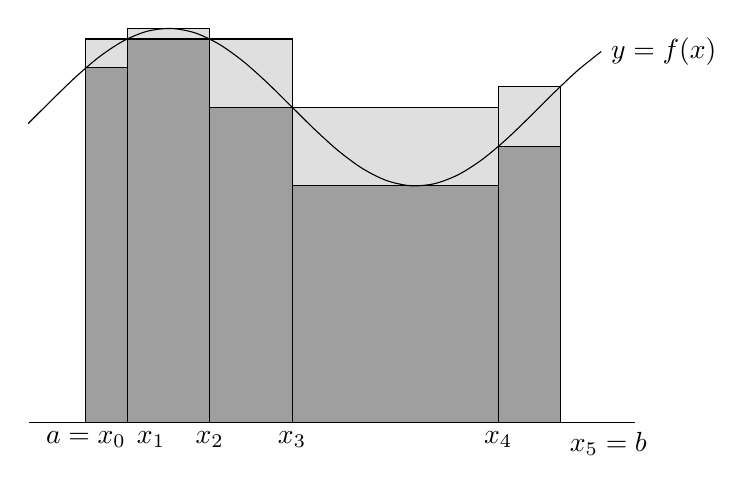
\begin{tikzpicture}
    \draw (-0.2,0)--(7.5,0);
    \filldraw[fill=lightgray!50,draw=black](pi/6,{sin(pi/6 r)+4}) rectangle (pi/3,{sin(pi/3 r)+4});
    \filldraw[fill=darkgray!50,draw=black](pi/6,0) rectangle (pi/3,{sin(pi/6 r)+4});
    \filldraw[fill=lightgray!50,draw=black](pi/3,{sin(pi/3 r)+4}) rectangle ({2*pi/3},5);
    \filldraw[fill=darkgray!50,draw=black](pi/3,0) rectangle ({2*pi/3},{sin(pi/3 r)+4});
    \filldraw[fill=lightgray!50,draw=black]({2*pi/3},{sin(pi r)+4}) rectangle (pi,{sin(2*pi/3 r)+4});
    \filldraw[fill=darkgray!50,draw=black]({2*pi/3},0) rectangle ({pi},{sin(pi r)+4});
    \filldraw[fill=lightgray!50,draw=black]({pi},3) rectangle ({11*pi/6},{sin(pi r)+4});
    \filldraw[fill=darkgray!50,draw=black]({pi},0) rectangle ({11*pi/6},3);
    \filldraw[fill=lightgray!50,draw=black]({11*pi/6},{sin(11*pi/6 r)+4}) rectangle ({25*pi/12},{sin(25*pi/12 r)+4});
    \filldraw[fill=darkgray!50,draw=black]({11*pi/6},0) rectangle ({25*pi/12},{sin(11*pi/6 r)+4});
    \draw (pi/6,0) node [below] {$a=x_0$};
    \draw (pi/3,0) node [below right] {$x_1$};
    \draw (2*pi/3,0) node [below] {$x_2$};
    \draw (pi,0) node [below] {$x_3$};
    \draw (11*pi/6,0) node [below] {$x_4$};
    \draw (25*pi/12,0) node [below right] {$x_5=b$};
    \draw [domain={-pi/15}:{27*pi/12},smooth] plot(\x, {sin(\x r) +4}) node [right]{$y=f(x)$};
  \end{tikzpicture}
  \caption{上方和と下方和}
  \end{figure}

\deref{上方和・下方和}において，$f$は$[a,b]$で有界だから，任意の$x \in [a,b]$に対して
\[
    m \leqq f(x) \leqq M
\]
となるような$m ,M \in \mathbb{R}$が存在する．

これより，
\[
    m(b-a) \leqq L(f,P) \leqq U(f,P) \leqq M(b-a)
\]
を得て，$L(f,P)$，$U(f,P)$はともに有界であることがわかった．

\begin{definition}{細分}{細分}
   区間$[a,b]$の分割$P^{\ast}$で，$P$の全ての分割が$P^{\ast}$の分割でもあるとき，$P^{\ast}$を$P$の細分という．
\end{definition}

\begin{prop}{細分と上方和・下方和}{細分と上方和・下方和}
  $P^{\ast}$を$P$の細分とするとき，
  \begin{align*}
    &U(f,P^{\ast})\leqq U(f,P),\\
    &L(f,P) \leqq L(f,P^{\ast})
  \end{align*}
  である．
\end{prop}

\begin{tleftbar}
  \begin{proof}
    上方和について証明する．

    分割$P$に，$x_{i-1} \leqq x^{\ast} \leqq x_i$を満たす点$x^{\ast}$を付け加えた細分を$P^{\ast}$とする．

    このとき，$U(f,P)$と$U(f,P^{\ast})$は，前者の$M_i (x_i-x_{i-1})$の項が後者だと
    \[
      M_i ' (x^{\ast}-x_{i-1}) +M_i '' (x_i-x^{\ast})
    \]
    に変わる点のみが異なる．ただしここで$M_i ' \coloneqq \sup_{x_{i-1} \leqq x \leqq x^{\ast}} f(x)$，
    $M_i '' \coloneqq \sup_{x^\ast \leqq x \leqq  x_i} f(x)$とした．

    $M_i,M_i ',M_i ''$の定義から
    \[
      M_i ' \leqq M_i , \quad M_i '' \leqq M_i
    \]
    なので，
    \begin{align*}
      M_i ' (x^{\ast}-x_{i-1}) +M_i '' (x_i-x^{\ast}) &\leqq M_i (x^{\ast}-x_{i-1}) + M_i(x_i -x^{\ast}) \\
      & = M_i (x_i - x_{i-1})
    \end{align*}
    となる．これよりただちに
    \[
      U(f,P^\ast) \leqq U(f,P)
    \]
    が従う．下方和についても同様である．これが証明すべきことであった．
  \end{proof}
\end{tleftbar}

\begin{prop}{}{}
  有界閉区間上の連続関数は積分可能である．
\end{prop}

\begin{tleftbar}
  \begin{proof}
    $f$を$[a,b]$上で連続な関数とする．このとき，任意の$\varepsilon >0$に対して，ある$\delta >0$が存在して，任意の$x,y \in [a,b]$に対して，
    $\abs{x-y}<\delta$のとき$\abs{f(x)-f(y)}<\varepsilon$となる．

    ここで，幅が$\delta$以下の分割$P=(a_i)_{i \in \{0,1,2,\ldots,n \}}$を考える．このとき，$[a_{i-1},a_i]$の点で
    \[
      f(x_i)=m_i (f,P),\quad f(y_i)=M_i (f,P)
    \]
    なるものが存在する．

    $\abs{x_i-y_i}\leqq \delta$であるから，$f(y_i)-f(x_i)<\varepsilon$となる．よって
    \[
      U(f,P)-L(f,P) = \sum_{i=1}^{n} ( f(y_i)-f(x_i) ) (a_i-a_{i-1}) <(b-a)\varepsilon
    \]
    となる．

    ここで，$L(f,P) \leqq L(f) \leqq U(f) \leqq U(f,P)$なので，$L(f)=U(f)$となり，$f$は積分可能である．これが証明すべきことであった．
  \end{proof}
\end{tleftbar}
\phantomsection
\subsection{定積分の性質}

\begin{prop}{}{}
  $f$が連続であるならば，
  \[
    \int_{a}^{b} f(x)\, dx = \int_{a}^{c} f(x)\, dx + \int_{c}^{b} f(x)\, dx
  \]
  が成立する．
\end{prop}

証明は省略する．

\begin{prop}{線型性}{線型性}
  連続関数$f,g$に対して，
  \[
    \int_{a}^{b} (kf(x)+lg(x))\, dx = k\int_{a}^{b} f(x)\, dx + l\int_{a}^{b} g(x)\, dx
  \]
  が成立する．
\end{prop}

証明は省略する．

\begin{definition}{リーマン和}{リーマン和}
  有界閉区間$[a,b]$上の有界関数$f$に対して，$P=(x_i)_{i \in \{0,1,2,\ldots,n\}}$を分割とする．

  さらには，$\xi_i \in [x_{i-1},x_i]$を適当に選ぶ．

  このとき，
  \[
    \sum_{i=1}^{n} f(\xi_i)(x_i - x_{i-1})
  \]
  を分割$P$と代表点$(\xi_i)_{i \in \{1,2,\ldots,n\} }$による$f$のリーマン和といい，
  \[
    R(f,P,\xi)
  \]
  と表す．
\end{definition}

\phantomsection
\part*{\texorpdfstring{積分($n$次元)}{積分(n次元)}}

\begin{definition}{}{}
  $n$次元の有界閉区間
  \begin{align*}
  I&=[a_1,b_1] \times [a_2,b_2] \times \cdots \times [a_n,b_n] \\
  & = \{ (x_1,x_2,\ldots,x_n) \mid a_i \leqq x_i \leqq b_i , i \in \{1,2,\dots,n \} \}
  \end{align*}
  の$n$次元体積を，
  \[
    v(I) = \prod_{i=1}^{n} (b_i-a_i)
  \]
  と定義する．
\end{definition}

\begin{definition}{}{}
  区間$I$に対して，集合 $D(I)$を
  \[
    D(I) = \{ (x_i)_{i \in \{0,1,\ldots,n \}} \mid a=x_0 < x_1<\dots < x_n =b , n \in \mathbb{N} \}
  \]
  とする．
\end{definition}

\begin{prop}{}{}
  $D(I)$は $(a,b)$の有限部分集合全体の集合$P((a,b))$と一対一に対応する．ただし，$a=b$のときは$a$を分点とする分割を考える．
\end{prop}

\begin{tleftbar}
  \begin{proof}
    写像$f$を
    \[
      f \colon D(I) \ni (x_i)_{i \in \{0,1,\ldots,n \}} \mapsto (x_i)_{i \in \{1,\ldots,n-1 \}} \in P((a,b))
    \]
    とする．このとき，$f$が全単射であることを示す．
    \begin{description}
      \item[単射であること] まず，$(x_i)_{i \in \{0,1,\ldots,n \}} \neq (y_i)_{i \in \{0,1,\ldots,n\}}$とする．
      このとき，ある$j \in \{0,1,\ldots,n \}$に対して，$ x_j \ne y_j $である．特に$ j \ne 0$かつ$j \ne n$のとき，
      \begin{align*}
        & (x_i)_{i \in \{1,2,\ldots,n-1 \}} \neq (y_i)_{i \in \{1,2,\ldots,n-1\}}, \\
        & \therefore ~ f((x_i)_{i \in \{0,1,\ldots,n \}}) \neq f((y_i)_{i \in \{0,1,\ldots,n\}})
      \end{align*}
      となるため，$f$は単射である．
      \item[全射であること] 任意の$(x_i)_{i \in \{1,\ldots,n-1 \}} \in P((a,b))$に対して，$a$および$b$を初項と末項に設定し，
      有限点列として
      \[
      (a,x_1,x_2,\ldots,x_{n-1},b)
      \]
      を考えると，これは$(x_0,x_1,\ldots,x_{n-1},x_n)$に等しい．ゆえにこのとき
      \[
      f((x_i)_{i \in \{0,1,\ldots,n\}})=(x_i)_{i \in \{1,\ldots,n-1 \}}
      \]
      となる$(x_i)_{i \in \{1,\ldots,n-1 \}} \in D(I)$が存在し，$f$は全射である．
    \end{description}
    以上の考察により，$f$は単射かつ全射，すなわち全単射である．これが証明すべきことであった．
  \end{proof}
\end{tleftbar}

\end{comment}
\newpage
\phantomsection

\part*{参考文献}

\noindent
本書は\cite{sugiura}，\cite{matsuzaka}，\cite{saito}を参考にした．

\medskip

\printbibliography[heading=none]

% 索引
% 参考文献の次のページ（偶数ページ）から索引を開始する．
% 通常の \part は右ページ開始だが，索引だけは右ページ送りを無効にする．

\clearpage
\thispagestyle{empty}
\setcounter{section}{6}
\renewcommand{\indexname}{索引}

\begingroup
  \makeatletter
  \def\part@newpage{\clearpage\thispagestyle{empty}}
  \makeatother
  \let\section\part
  \pagestyle{empty}
  \printindex
\endgroup

% 裏表紙が \BookTotalPages ページ目（偶数ページ）に来るよう白紙を補充する．
% 末尾 2 ページ＝裏表紙の裏（白紙）＋裏表紙．
% \ReadonlyShipoutCounter は表紙を含めた出力済みの物理ページ数．
\clearpage
\pagestyle{empty}
\makeatletter
\@tempcnta=\numexpr\BookTotalPages-2-\ReadonlyShipoutCounter\relax
\ifnum\@tempcnta<0
  \PackageWarningNoLine{製本}{本文が \BookTotalPages\space ページを超えています}
\fi
\loop\ifnum\@tempcnta>0
  \thispagestyle{empty}\null\clearpage
  \advance\@tempcnta\m@ne
\repeat
\makeatother
\MathNoteBackCoverBlankfalse

\MathNoteBackCover{Analysis}{2026 Edition}

\end{document}
